% Options for packages loaded elsewhere
\PassOptionsToPackage{unicode}{hyperref}
\PassOptionsToPackage{hyphens}{url}
\PassOptionsToPackage{dvipsnames,svgnames*,x11names*}{xcolor}
%
\documentclass[
]{article}
\usepackage{lmodern}
\usepackage{amssymb,amsmath}
\usepackage{ifxetex,ifluatex}
\ifnum 0\ifxetex 1\fi\ifluatex 1\fi=0 % if pdftex
  \usepackage[T1]{fontenc}
  \usepackage[utf8]{inputenc}
  \usepackage{textcomp} % provide euro and other symbols
\else % if luatex or xetex
  \usepackage{unicode-math}
  \defaultfontfeatures{Scale=MatchLowercase}
  \defaultfontfeatures[\rmfamily]{Ligatures=TeX,Scale=1}
\fi
% Use upquote if available, for straight quotes in verbatim environments
\IfFileExists{upquote.sty}{\usepackage{upquote}}{}
\IfFileExists{microtype.sty}{% use microtype if available
  \usepackage[]{microtype}
  \UseMicrotypeSet[protrusion]{basicmath} % disable protrusion for tt fonts
}{}
\makeatletter
\@ifundefined{KOMAClassName}{% if non-KOMA class
  \IfFileExists{parskip.sty}{%
    \usepackage{parskip}
  }{% else
    \setlength{\parindent}{0pt}
    \setlength{\parskip}{6pt plus 2pt minus 1pt}}
}{% if KOMA class
  \KOMAoptions{parskip=half}}
\makeatother
\usepackage{xcolor}
\IfFileExists{xurl.sty}{\usepackage{xurl}}{} % add URL line breaks if available
\IfFileExists{bookmark.sty}{\usepackage{bookmark}}{\usepackage{hyperref}}
\hypersetup{
  pdftitle={Data Exploration: Contextual Influences},
  pdfauthor={Your name here},
  colorlinks=true,
  linkcolor=Maroon,
  filecolor=Maroon,
  citecolor=Blue,
  urlcolor=blue,
  pdfcreator={LaTeX via pandoc}}
\urlstyle{same} % disable monospaced font for URLs
\usepackage[margin=1in]{geometry}
\usepackage{color}
\usepackage{fancyvrb}
\newcommand{\VerbBar}{|}
\newcommand{\VERB}{\Verb[commandchars=\\\{\}]}
\DefineVerbatimEnvironment{Highlighting}{Verbatim}{commandchars=\\\{\}}
% Add ',fontsize=\small' for more characters per line
\usepackage{framed}
\definecolor{shadecolor}{RGB}{248,248,248}
\newenvironment{Shaded}{\begin{snugshade}}{\end{snugshade}}
\newcommand{\AlertTok}[1]{\textcolor[rgb]{0.94,0.16,0.16}{#1}}
\newcommand{\AnnotationTok}[1]{\textcolor[rgb]{0.56,0.35,0.01}{\textbf{\textit{#1}}}}
\newcommand{\AttributeTok}[1]{\textcolor[rgb]{0.77,0.63,0.00}{#1}}
\newcommand{\BaseNTok}[1]{\textcolor[rgb]{0.00,0.00,0.81}{#1}}
\newcommand{\BuiltInTok}[1]{#1}
\newcommand{\CharTok}[1]{\textcolor[rgb]{0.31,0.60,0.02}{#1}}
\newcommand{\CommentTok}[1]{\textcolor[rgb]{0.56,0.35,0.01}{\textit{#1}}}
\newcommand{\CommentVarTok}[1]{\textcolor[rgb]{0.56,0.35,0.01}{\textbf{\textit{#1}}}}
\newcommand{\ConstantTok}[1]{\textcolor[rgb]{0.00,0.00,0.00}{#1}}
\newcommand{\ControlFlowTok}[1]{\textcolor[rgb]{0.13,0.29,0.53}{\textbf{#1}}}
\newcommand{\DataTypeTok}[1]{\textcolor[rgb]{0.13,0.29,0.53}{#1}}
\newcommand{\DecValTok}[1]{\textcolor[rgb]{0.00,0.00,0.81}{#1}}
\newcommand{\DocumentationTok}[1]{\textcolor[rgb]{0.56,0.35,0.01}{\textbf{\textit{#1}}}}
\newcommand{\ErrorTok}[1]{\textcolor[rgb]{0.64,0.00,0.00}{\textbf{#1}}}
\newcommand{\ExtensionTok}[1]{#1}
\newcommand{\FloatTok}[1]{\textcolor[rgb]{0.00,0.00,0.81}{#1}}
\newcommand{\FunctionTok}[1]{\textcolor[rgb]{0.00,0.00,0.00}{#1}}
\newcommand{\ImportTok}[1]{#1}
\newcommand{\InformationTok}[1]{\textcolor[rgb]{0.56,0.35,0.01}{\textbf{\textit{#1}}}}
\newcommand{\KeywordTok}[1]{\textcolor[rgb]{0.13,0.29,0.53}{\textbf{#1}}}
\newcommand{\NormalTok}[1]{#1}
\newcommand{\OperatorTok}[1]{\textcolor[rgb]{0.81,0.36,0.00}{\textbf{#1}}}
\newcommand{\OtherTok}[1]{\textcolor[rgb]{0.56,0.35,0.01}{#1}}
\newcommand{\PreprocessorTok}[1]{\textcolor[rgb]{0.56,0.35,0.01}{\textit{#1}}}
\newcommand{\RegionMarkerTok}[1]{#1}
\newcommand{\SpecialCharTok}[1]{\textcolor[rgb]{0.00,0.00,0.00}{#1}}
\newcommand{\SpecialStringTok}[1]{\textcolor[rgb]{0.31,0.60,0.02}{#1}}
\newcommand{\StringTok}[1]{\textcolor[rgb]{0.31,0.60,0.02}{#1}}
\newcommand{\VariableTok}[1]{\textcolor[rgb]{0.00,0.00,0.00}{#1}}
\newcommand{\VerbatimStringTok}[1]{\textcolor[rgb]{0.31,0.60,0.02}{#1}}
\newcommand{\WarningTok}[1]{\textcolor[rgb]{0.56,0.35,0.01}{\textbf{\textit{#1}}}}
\usepackage{longtable,booktabs}
% Correct order of tables after \paragraph or \subparagraph
\usepackage{etoolbox}
\makeatletter
\patchcmd\longtable{\par}{\if@noskipsec\mbox{}\fi\par}{}{}
\makeatother
% Allow footnotes in longtable head/foot
\IfFileExists{footnotehyper.sty}{\usepackage{footnotehyper}}{\usepackage{footnote}}
\makesavenoteenv{longtable}
\usepackage{graphicx,grffile}
\makeatletter
\def\maxwidth{\ifdim\Gin@nat@width>\linewidth\linewidth\else\Gin@nat@width\fi}
\def\maxheight{\ifdim\Gin@nat@height>\textheight\textheight\else\Gin@nat@height\fi}
\makeatother
% Scale images if necessary, so that they will not overflow the page
% margins by default, and it is still possible to overwrite the defaults
% using explicit options in \includegraphics[width, height, ...]{}
\setkeys{Gin}{width=\maxwidth,height=\maxheight,keepaspectratio}
% Set default figure placement to htbp
\makeatletter
\def\fps@figure{htbp}
\makeatother
\setlength{\emergencystretch}{3em} % prevent overfull lines
\providecommand{\tightlist}{%
  \setlength{\itemsep}{0pt}\setlength{\parskip}{0pt}}
\setcounter{secnumdepth}{-\maxdimen} % remove section numbering
\usepackage{array}
\usepackage{caption}
\usepackage{graphicx}
\usepackage{siunitx}
\usepackage[normalem]{ulem}
\usepackage{colortbl}
\usepackage{multirow}
\usepackage{hhline}
\usepackage{calc}
\usepackage{tabularx}
\usepackage{threeparttable}
\usepackage{wrapfig}
\usepackage{adjustbox}
\usepackage{hyperref}

\title{Data Exploration: Contextual Influences}
\author{Your name here}
\date{November 11, 2021}

\begin{document}
\maketitle

In this Data Exploration assignment we will again be exploring the
Nationscape dataset (Tausanovitch and Vavreck 2020), which was used in
Reny and Newman's (2021) study of the effecs of the protests after
George Floyd's killing.

Unlike previous assignments, however, you will be asked to take a bigger
role in defining the research question and identifying the specific data
that you would need to use. \emph{This is practice for operationalizing
questions of the type you will do for your research project.}

Throughout the assignment, we will provide a running example of how you
might approach the tasks. For you own work, please do not use either
this example or the Geroge Floyd protests.

\textbf{Note: Because this assignment is a bit different, you are
require to do all of the questions (although non-data science students
can skip question 7). This is to ensure that you have enough material
for you blog post.}

If you have a question about any part of this assignment, please ask!
Note that the actionable part of each question is \textbf{bolded}.

\hypertarget{developing-a-research-question-about-contextual-influences}{%
\section{Developing a Research Question about Contextual
Influences}\label{developing-a-research-question-about-contextual-influences}}

\textbf{Data Details:}

\begin{itemize}
\item
  File Name: \texttt{vars\_data.xlsx}
\item
  Source: This file shows what variables are covered in each wave of the
  Nationscape Data Set (Tausanovitch and Vavreck 2020). We will be using
  data from the survey itself in other parts of the exercise, but which
  specific files and variables will be up to you! Therefore, we don't
  present them in depth here.
\end{itemize}

\begin{longtable}[]{@{}ll@{}}
\toprule
\begin{minipage}[b]{0.33\columnwidth}\raggedright
Variable Name\strut
\end{minipage} & \begin{minipage}[b]{0.61\columnwidth}\raggedright
Variable Description\strut
\end{minipage}\tabularnewline
\midrule
\endhead
\begin{minipage}[t]{0.33\columnwidth}\raggedright
\texttt{Date}\strut
\end{minipage} & \begin{minipage}[t]{0.61\columnwidth}\raggedright
The date of the wave of the Nationscape survey\strut
\end{minipage}\tabularnewline
\begin{minipage}[t]{0.33\columnwidth}\raggedright
\texttt{response\_id}\strut
\end{minipage} & \begin{minipage}[t]{0.61\columnwidth}\raggedright
This and all other variables are the names of variables in the
Nationscape data; the cells are 1 if that variable was included in that
week's survey and 0 otherwise\strut
\end{minipage}\tabularnewline
\bottomrule
\end{longtable}

\begin{Shaded}
\begin{Highlighting}[]
\CommentTok{#Load the data summarizing variable availability}
\NormalTok{NationscapeVars_}\DecValTok{1}\NormalTok{ <-}\StringTok{ }\KeywordTok{read_xlsx}\NormalTok{(}\StringTok{'vars_data.xlsx'}\NormalTok{,}\DataTypeTok{sheet =} \DecValTok{1}\NormalTok{) }\CommentTok{#we're using the read_xlsx function from the readxl package, which lets you specify which sheet to upload if you are using Excel data with multiple sheets}
\NormalTok{NationscapeVars_}\DecValTok{2}\NormalTok{ <-}\StringTok{ }\KeywordTok{read_xlsx}\NormalTok{(}\StringTok{'vars_data.xlsx'}\NormalTok{,}\DataTypeTok{sheet =} \DecValTok{2}\NormalTok{)}
\end{Highlighting}
\end{Shaded}

Now let's get the data from two sheets into one data set.

\begin{Shaded}
\begin{Highlighting}[]
\NormalTok{NationscapeVars <-}\StringTok{ }\KeywordTok{full_join}\NormalTok{(NationscapeVars_}\DecValTok{1}\NormalTok{,NationscapeVars_}\DecValTok{2}\NormalTok{) }\OperatorTok\StringTok{ }\CommentTok{# the full_join function keeps all rows in both objects and all columns}
\StringTok{  }\KeywordTok{replace}\NormalTok{(}\KeywordTok{is.na}\NormalTok{(.),}\DecValTok{0}\NormalTok{) }\CommentTok{# since we know that the NAs generated in the last command weren't asked in the weeks that show up as NA, we can replace NAs with 0s}
\end{Highlighting}
\end{Shaded}

\begin{verbatim}
## Joining, by = c("Date", "response_id", "start_date", "right_track", "economy_better", "interest", "registration", "news_sources_facebook", "news_sources_cnn", "news_sources_msnbc", "news_sources_fox", "news_sources_network", "news_sources_localtv", "news_sources_telemundo", "news_sources_npr", "news_sources_amtalk", "news_sources_new_york_times", "news_sources_local_newspaper", "news_sources_other", "news_sources_other_TEXT", "pres_approval", "vote_intention", "vote_2016", "vote_2016_other_text", "consider_trump", "not_trump", "primary_party", "group_favorability_whites", "group_favorability_blacks", "group_favorability_latinos", "group_favorability_asians", "group_favorability_socialists", "group_favorability_muslims", "group_favorability_labor_unions", "group_favorability_the_police", "group_favorability_undocumented", "group_favorability_lgbt", "group_favorability_republicans", "group_favorability_democrats", "cand_favorability_trump", "cand_favorability_obama", "cand_favorability_biden", "cand_favorability_harris", "cand_favorability_buttigieg", "cand_favorability_warren", "cand_favorability_sanders", "dem_vote_intent", "rank_dems_1", "rank_dems_2", "rank_dems_3", "replace_trump", "house_intent", "senate_intent", "governor_intent", "trump_biden", "trump_sanders", "trump_warren", "trump_buttigieg", "pence_biden", "pence_buttigieg", "pence_sanders", "pence_warren", "cand_truth_donald_trump", "cand_truth_elizabeth_warren", "cand_truth_joe_biden", "cand_truth_bernie_sanders", "cand_truth_pete_buttigieg", "cand_facts_donald_trump", "cand_facts_elizabeth_warren", "cand_facts_joe_biden", "cand_facts_bernie_sanders", "cand_facts_pete_buttigieg", "racial_attitudes_tryhard", "racial_attitudes_generations", "racial_attitudes_marry", "racial_attitudes_date", "gender_attitudes_maleboss", "gender_attitudes_logical", "gender_attitudes_opportunity", "gender_attitudes_complain", "discrimination_blacks", "discrimination_whites", "discrimination_muslims", "discrimination_christians", "discrimination_women", "discrimination_men", "sen_knowledge", "sc_knowledge", "pid3", "pid7_legacy", "strength_democrat", "strength_republican", "lean_independent", "ideo5", "employment", "employment_other_text", "foreign_born", "language", "religion", "religion_other_text", "is_evangelical", "orientation_group", "in_union", "household_gun_owner", "wall", "cap_carbon", "environment", "guns_bg", "mctaxes", "estate_tax", "raise_upper_tax", "college", "abortion_waiting", "abortion_never", "abortion_conditions", "late_term_abortion", "abortion_insurance", "guaranteed_jobs", "green_new_deal", "gun_registry", "immigration_separation", "immigration_system", "immigration_wire", "impeach_trump", "israel", "marijuana", "maternityleave", "medicare_for_all", "military_size", "minwage", "muslimban", "oil_and_gas", "reparations", "right_to_work", "ten_commandments", "trade", "trans_military", "uctaxes2", "vouchers", "gov_insurance", "public_option", "health_subsidies", "path_to_citizenship", "dreamers", "deportation", "ban_guns", "ban_assault_rifles", "limit_magazines", "age", "gender", "census_region", "hispanic", "race_ethnicity", "household_income", "education", "state", "congress_district", "weight", "dem_vote_intent_TEXT", "rep_vote_prim", "rep_vote_prim_TEXT", "group_favorability_evangelicals", "group_favorability_white_men", "fc_smallgov", "fc_trad_val", "statements_protect_traditions", "statements_defense_burden", "statements_trade_effects", "statements_christianity_assault", "statements_gender_identity", "statements_american_loss", "statements_imm_assimilate", "statements_gun_rights", "statements_confront_china", "statements_foreign_interests", "abortion_any_time", "abolish_priv_insurance", "china_tariffs", "criminal_immigration", "immigration_insurance", "primary_sen_barrasso", "primary_sen_blackburn", "primary_sen_blunt", "primary_sen_cassidy", "primary_sen_collins", "primary_sen_cornyn", "primary_sen_cotton", "primary_sen_daines", "primary_sen_ernst", "primary_sen_gardner", "primary_sen_graham", "primary_sen_hoeven", "primary_sen_hydesmith", "primary_sen_inhofe", "primary_sen_lee", "primary_sen_mcconnell", "primary_sen_mcsally", "primary_sen_moorecapito", "primary_sen_moran", "primary_sen_perdue", "primary_sen_portman", "primary_sen_risch", "primary_sen_rounds", "primary_sen_rubio", "primary_sen_sasse", "primary_sen_shelby", "primary_sen_sullivan", "primary_sen_tillis", "primary_sen_toomey", "primary_sen_young", "primary_sen_boozman", "primary_sen_braun", "primary_sen_cramer", "primary_sen_crapo", "primary_sen_cruz", "primary_sen_fischer", "primary_sen_grassley", "primary_sen_hawley", "primary_sen_lankford", "primary_sen_murkowski", "primary_sen_neelykennedy", "primary_sen_paul", "primary_sen_romney", "primary_sen_scott_rick", "primary_sen_scott_tim", "primary_sen_thune", "primary_sen_wicker", "extra_group_favor_demcong", "extra_group_favor_repcong", "extra_group_identity_race", "extra_group_identity_partyID", "extra_group_id_relig_belief", "extra_group_identity_local_comm", "extra_group_identity_close_fam", "extra_group_id_being_american", "extra_n_children", "extra_n_adults", "extra_housing", "extra_party_ideo_rate_dem", "extra_party_ideo_rate_rep", "extra_party_ideo_dem_desire", "extra_party_ideo_rep_desire", "extra_foreign_interf", "extra_foreign_help", "extra_foreign_effect", "extra_dem_prim", "extra_rep_prim", "extra_dem_prim_cand", "extra_rep_prim_cand", "extra_trump_cares_me", "extra_trump_cares_poor", "extra_trump_cares_mid_class", "extra_trump_cares_wealthy", "extra_biden_cares_me", "extra_biden_cares_poor", "extra_biden_cares_mid_class", "extra_biden_cares_wealthy", "group_favorability_jews", "discrimination_jews")
\end{verbatim}

\hypertarget{question-1}{%
\subsection{Question 1}\label{question-1}}

Contextual influences are all about the fleeting events that shift our
attitudes and behavior. These can be something we personally experience,
like encountering people on the street (Sands 2017) or voting at a
school (Berger et al.~2008). But they can also be events we are exposed
to by press coverage like Supreme Court decision (Tankard and Paluck
2017) or even emotions evoked by press coverage (as was experimentally
modeled by Zeitzoff 2014). For this exercise we will think about events
that people in a given state or across the country would plausibly have
been exposed to via news coverage. \textbf{Think about events that
happened between July 2019 and July 2020. Maybe this is something that
made national news or maybe it was something that received a lot of
coverage in your home state or region. Write down an example or two that
you might be interested in considering. Use
\href{https://trends.google.com/trends/?geo=US}{Google Trends} to
confirm that there was a spike in interest, as demonstrated by an
increase in Google searches, in your event and include a screenshot or a
hyperlink to your results.} Try entering a relevant search term and then
using a ``Custom time range'' (one of the drop down options instead of
the default "``Past 12 months'') to make your visualization.

\hypertarget{my-question}{%
\subsection{My Question}\label{my-question}}

I'm going to look at the first impeachment of Pres.~Donald Trump;
\href{https://trends.google.com/trends/explore?date=2019-07-01\%202020-07-31\&geo=US\&q=impeachment}{Google
Trends} confirms a big spike around December 18, when the House voted to
impeach on two articles.

\hypertarget{question-2}{%
\subsection{Question 2}\label{question-2}}

Think about some outcomes of interest to you that might have been
affected by the contextual influence of the event that you chose. Look
in the Nationscape data for variables that fit your outcomes or are
reasonable proxies for those outcomes. The variable names in the data
you have loaded are pretty informative, but use the full data folder you
downloaded earlier to look in the codebooks for more complete
descriptions of the variables and how they are measured. There is a
codebook in each week's folder; you can look at any week's codebook to
get a sense of the variables that are common across the survey waves.
\textbf{Make sure that your variables are present in the data for the
time period in which you want to look for contextual effects. Present
these results in a plot.}

\begin{Shaded}
\begin{Highlighting}[]
\NormalTok{NationscapeVars }\OperatorTok
\StringTok{  }\KeywordTok{select}\NormalTok{(Date, pres_approval, consider_trump, pid7_legacy, ideo5, muslimban, age) }\OperatorTok
\StringTok{  }\KeywordTok{mutate}\NormalTok{(}\DataTypeTok{date =} \KeywordTok{as.character}\NormalTok{(Date)) }\OperatorTok
\StringTok{  }\KeywordTok{filter}\NormalTok{(date }\OperatorTok{==}\StringTok{ "2019-12-05"} \OperatorTok{|}\StringTok{ }\NormalTok{date }\OperatorTok{==}\StringTok{ "2019-12-12"} \OperatorTok{|}\StringTok{ }\NormalTok{date }\OperatorTok{==}\StringTok{ "2019-12-19"} \OperatorTok{|}\StringTok{ }\NormalTok{date }\OperatorTok{==}\StringTok{ "2019-12-26"} \OperatorTok{|}\StringTok{ }\NormalTok{date }\OperatorTok{==}\StringTok{ "2020-01-02"}\NormalTok{)}
\end{Highlighting}
\end{Shaded}

 
  \providecommand{\huxb}[2]{\arrayrulecolor[RGB]{#1}\global\arrayrulewidth=#2pt}
  \providecommand{\huxvb}[2]{\color[RGB]{#1}\vrule width #2pt}
  \providecommand{\huxtpad}[1]{\rule{0pt}{#1}}
  \providecommand{\huxbpad}[1]{\rule[-#1]{0pt}{#1}}

\begin{table}[ht]
\begin{centerbox}
\begin{threeparttable}
 \label{tab:q2}
\setlength{\tabcolsep}{0pt}
\begin{tabular}{l l l l l l l l}


\hhline{>{\huxb{0, 0, 0}{0.4}}->{\huxb{0, 0, 0}{0.4}}->{\huxb{0, 0, 0}{0.4}}->{\huxb{0, 0, 0}{0.4}}->{\huxb{0, 0, 0}{0.4}}->{\huxb{0, 0, 0}{0.4}}->{\huxb{0, 0, 0}{0.4}}->{\huxb{0, 0, 0}{0.4}}-}
\arrayrulecolor{black}

\multicolumn{1}{!{\huxvb{0, 0, 0}{0.4}}r!{\huxvb{0, 0, 0}{0}}}{\huxtpad{6pt + 1em}\raggedleft \hspace{6pt} \textbf{Date} \hspace{6pt}\huxbpad{6pt}} &
\multicolumn{1}{r!{\huxvb{0, 0, 0}{0}}}{\huxtpad{6pt + 1em}\raggedleft \hspace{6pt} \textbf{pres\_approval} \hspace{6pt}\huxbpad{6pt}} &
\multicolumn{1}{r!{\huxvb{0, 0, 0}{0}}}{\huxtpad{6pt + 1em}\raggedleft \hspace{6pt} \textbf{consider\_trump} \hspace{6pt}\huxbpad{6pt}} &
\multicolumn{1}{r!{\huxvb{0, 0, 0}{0}}}{\huxtpad{6pt + 1em}\raggedleft \hspace{6pt} \textbf{pid7\_legacy} \hspace{6pt}\huxbpad{6pt}} &
\multicolumn{1}{r!{\huxvb{0, 0, 0}{0}}}{\huxtpad{6pt + 1em}\raggedleft \hspace{6pt} \textbf{ideo5} \hspace{6pt}\huxbpad{6pt}} &
\multicolumn{1}{r!{\huxvb{0, 0, 0}{0}}}{\huxtpad{6pt + 1em}\raggedleft \hspace{6pt} \textbf{muslimban} \hspace{6pt}\huxbpad{6pt}} &
\multicolumn{1}{r!{\huxvb{0, 0, 0}{0}}}{\huxtpad{6pt + 1em}\raggedleft \hspace{6pt} \textbf{age} \hspace{6pt}\huxbpad{6pt}} &
\multicolumn{1}{l!{\huxvb{0, 0, 0}{0.4}}}{\huxtpad{6pt + 1em}\raggedright \hspace{6pt} \textbf{date} \hspace{6pt}\huxbpad{6pt}} \tabularnewline[-0.5pt]


\hhline{>{\huxb{0, 0, 0}{0.4}}->{\huxb{0, 0, 0}{0.4}}->{\huxb{0, 0, 0}{0.4}}->{\huxb{0, 0, 0}{0.4}}->{\huxb{0, 0, 0}{0.4}}->{\huxb{0, 0, 0}{0.4}}->{\huxb{0, 0, 0}{0.4}}->{\huxb{0, 0, 0}{0.4}}-}
\arrayrulecolor{black}

\multicolumn{1}{!{\huxvb{0, 0, 0}{0.4}}r!{\huxvb{0, 0, 0}{0}}}{\cellcolor[RGB]{242, 242, 242}\huxtpad{6pt + 1em}\raggedleft \hspace{6pt} 2019-12-05 \hspace{6pt}\huxbpad{6pt}} &
\multicolumn{1}{r!{\huxvb{0, 0, 0}{0}}}{\cellcolor[RGB]{242, 242, 242}\huxtpad{6pt + 1em}\raggedleft \hspace{6pt} 1 \hspace{6pt}\huxbpad{6pt}} &
\multicolumn{1}{r!{\huxvb{0, 0, 0}{0}}}{\cellcolor[RGB]{242, 242, 242}\huxtpad{6pt + 1em}\raggedleft \hspace{6pt} 1 \hspace{6pt}\huxbpad{6pt}} &
\multicolumn{1}{r!{\huxvb{0, 0, 0}{0}}}{\cellcolor[RGB]{242, 242, 242}\huxtpad{6pt + 1em}\raggedleft \hspace{6pt} 1 \hspace{6pt}\huxbpad{6pt}} &
\multicolumn{1}{r!{\huxvb{0, 0, 0}{0}}}{\cellcolor[RGB]{242, 242, 242}\huxtpad{6pt + 1em}\raggedleft \hspace{6pt} 1 \hspace{6pt}\huxbpad{6pt}} &
\multicolumn{1}{r!{\huxvb{0, 0, 0}{0}}}{\cellcolor[RGB]{242, 242, 242}\huxtpad{6pt + 1em}\raggedleft \hspace{6pt} 1 \hspace{6pt}\huxbpad{6pt}} &
\multicolumn{1}{r!{\huxvb{0, 0, 0}{0}}}{\cellcolor[RGB]{242, 242, 242}\huxtpad{6pt + 1em}\raggedleft \hspace{6pt} 1 \hspace{6pt}\huxbpad{6pt}} &
\multicolumn{1}{l!{\huxvb{0, 0, 0}{0.4}}}{\cellcolor[RGB]{242, 242, 242}\huxtpad{6pt + 1em}\raggedright \hspace{6pt} 2019-12-05 \hspace{6pt}\huxbpad{6pt}} \tabularnewline[-0.5pt]


\hhline{>{\huxb{0, 0, 0}{0.4}}|>{\huxb{0, 0, 0}{0.4}}|}
\arrayrulecolor{black}

\multicolumn{1}{!{\huxvb{0, 0, 0}{0.4}}r!{\huxvb{0, 0, 0}{0}}}{\huxtpad{6pt + 1em}\raggedleft \hspace{6pt} 2019-12-12 \hspace{6pt}\huxbpad{6pt}} &
\multicolumn{1}{r!{\huxvb{0, 0, 0}{0}}}{\huxtpad{6pt + 1em}\raggedleft \hspace{6pt} 1 \hspace{6pt}\huxbpad{6pt}} &
\multicolumn{1}{r!{\huxvb{0, 0, 0}{0}}}{\huxtpad{6pt + 1em}\raggedleft \hspace{6pt} 1 \hspace{6pt}\huxbpad{6pt}} &
\multicolumn{1}{r!{\huxvb{0, 0, 0}{0}}}{\huxtpad{6pt + 1em}\raggedleft \hspace{6pt} 1 \hspace{6pt}\huxbpad{6pt}} &
\multicolumn{1}{r!{\huxvb{0, 0, 0}{0}}}{\huxtpad{6pt + 1em}\raggedleft \hspace{6pt} 1 \hspace{6pt}\huxbpad{6pt}} &
\multicolumn{1}{r!{\huxvb{0, 0, 0}{0}}}{\huxtpad{6pt + 1em}\raggedleft \hspace{6pt} 1 \hspace{6pt}\huxbpad{6pt}} &
\multicolumn{1}{r!{\huxvb{0, 0, 0}{0}}}{\huxtpad{6pt + 1em}\raggedleft \hspace{6pt} 1 \hspace{6pt}\huxbpad{6pt}} &
\multicolumn{1}{l!{\huxvb{0, 0, 0}{0.4}}}{\huxtpad{6pt + 1em}\raggedright \hspace{6pt} 2019-12-12 \hspace{6pt}\huxbpad{6pt}} \tabularnewline[-0.5pt]


\hhline{>{\huxb{0, 0, 0}{0.4}}|>{\huxb{0, 0, 0}{0.4}}|}
\arrayrulecolor{black}

\multicolumn{1}{!{\huxvb{0, 0, 0}{0.4}}r!{\huxvb{0, 0, 0}{0}}}{\cellcolor[RGB]{242, 242, 242}\huxtpad{6pt + 1em}\raggedleft \hspace{6pt} 2019-12-19 \hspace{6pt}\huxbpad{6pt}} &
\multicolumn{1}{r!{\huxvb{0, 0, 0}{0}}}{\cellcolor[RGB]{242, 242, 242}\huxtpad{6pt + 1em}\raggedleft \hspace{6pt} 1 \hspace{6pt}\huxbpad{6pt}} &
\multicolumn{1}{r!{\huxvb{0, 0, 0}{0}}}{\cellcolor[RGB]{242, 242, 242}\huxtpad{6pt + 1em}\raggedleft \hspace{6pt} 1 \hspace{6pt}\huxbpad{6pt}} &
\multicolumn{1}{r!{\huxvb{0, 0, 0}{0}}}{\cellcolor[RGB]{242, 242, 242}\huxtpad{6pt + 1em}\raggedleft \hspace{6pt} 1 \hspace{6pt}\huxbpad{6pt}} &
\multicolumn{1}{r!{\huxvb{0, 0, 0}{0}}}{\cellcolor[RGB]{242, 242, 242}\huxtpad{6pt + 1em}\raggedleft \hspace{6pt} 1 \hspace{6pt}\huxbpad{6pt}} &
\multicolumn{1}{r!{\huxvb{0, 0, 0}{0}}}{\cellcolor[RGB]{242, 242, 242}\huxtpad{6pt + 1em}\raggedleft \hspace{6pt} 1 \hspace{6pt}\huxbpad{6pt}} &
\multicolumn{1}{r!{\huxvb{0, 0, 0}{0}}}{\cellcolor[RGB]{242, 242, 242}\huxtpad{6pt + 1em}\raggedleft \hspace{6pt} 1 \hspace{6pt}\huxbpad{6pt}} &
\multicolumn{1}{l!{\huxvb{0, 0, 0}{0.4}}}{\cellcolor[RGB]{242, 242, 242}\huxtpad{6pt + 1em}\raggedright \hspace{6pt} 2019-12-19 \hspace{6pt}\huxbpad{6pt}} \tabularnewline[-0.5pt]


\hhline{>{\huxb{0, 0, 0}{0.4}}|>{\huxb{0, 0, 0}{0.4}}|}
\arrayrulecolor{black}

\multicolumn{1}{!{\huxvb{0, 0, 0}{0.4}}r!{\huxvb{0, 0, 0}{0}}}{\huxtpad{6pt + 1em}\raggedleft \hspace{6pt} 2019-12-26 \hspace{6pt}\huxbpad{6pt}} &
\multicolumn{1}{r!{\huxvb{0, 0, 0}{0}}}{\huxtpad{6pt + 1em}\raggedleft \hspace{6pt} 1 \hspace{6pt}\huxbpad{6pt}} &
\multicolumn{1}{r!{\huxvb{0, 0, 0}{0}}}{\huxtpad{6pt + 1em}\raggedleft \hspace{6pt} 1 \hspace{6pt}\huxbpad{6pt}} &
\multicolumn{1}{r!{\huxvb{0, 0, 0}{0}}}{\huxtpad{6pt + 1em}\raggedleft \hspace{6pt} 1 \hspace{6pt}\huxbpad{6pt}} &
\multicolumn{1}{r!{\huxvb{0, 0, 0}{0}}}{\huxtpad{6pt + 1em}\raggedleft \hspace{6pt} 1 \hspace{6pt}\huxbpad{6pt}} &
\multicolumn{1}{r!{\huxvb{0, 0, 0}{0}}}{\huxtpad{6pt + 1em}\raggedleft \hspace{6pt} 1 \hspace{6pt}\huxbpad{6pt}} &
\multicolumn{1}{r!{\huxvb{0, 0, 0}{0}}}{\huxtpad{6pt + 1em}\raggedleft \hspace{6pt} 1 \hspace{6pt}\huxbpad{6pt}} &
\multicolumn{1}{l!{\huxvb{0, 0, 0}{0.4}}}{\huxtpad{6pt + 1em}\raggedright \hspace{6pt} 2019-12-26 \hspace{6pt}\huxbpad{6pt}} \tabularnewline[-0.5pt]


\hhline{>{\huxb{0, 0, 0}{0.4}}|>{\huxb{0, 0, 0}{0.4}}|}
\arrayrulecolor{black}

\multicolumn{1}{!{\huxvb{0, 0, 0}{0.4}}r!{\huxvb{0, 0, 0}{0}}}{\cellcolor[RGB]{242, 242, 242}\huxtpad{6pt + 1em}\raggedleft \hspace{6pt} 2020-01-02 \hspace{6pt}\huxbpad{6pt}} &
\multicolumn{1}{r!{\huxvb{0, 0, 0}{0}}}{\cellcolor[RGB]{242, 242, 242}\huxtpad{6pt + 1em}\raggedleft \hspace{6pt} 1 \hspace{6pt}\huxbpad{6pt}} &
\multicolumn{1}{r!{\huxvb{0, 0, 0}{0}}}{\cellcolor[RGB]{242, 242, 242}\huxtpad{6pt + 1em}\raggedleft \hspace{6pt} 1 \hspace{6pt}\huxbpad{6pt}} &
\multicolumn{1}{r!{\huxvb{0, 0, 0}{0}}}{\cellcolor[RGB]{242, 242, 242}\huxtpad{6pt + 1em}\raggedleft \hspace{6pt} 1 \hspace{6pt}\huxbpad{6pt}} &
\multicolumn{1}{r!{\huxvb{0, 0, 0}{0}}}{\cellcolor[RGB]{242, 242, 242}\huxtpad{6pt + 1em}\raggedleft \hspace{6pt} 1 \hspace{6pt}\huxbpad{6pt}} &
\multicolumn{1}{r!{\huxvb{0, 0, 0}{0}}}{\cellcolor[RGB]{242, 242, 242}\huxtpad{6pt + 1em}\raggedleft \hspace{6pt} 1 \hspace{6pt}\huxbpad{6pt}} &
\multicolumn{1}{r!{\huxvb{0, 0, 0}{0}}}{\cellcolor[RGB]{242, 242, 242}\huxtpad{6pt + 1em}\raggedleft \hspace{6pt} 1 \hspace{6pt}\huxbpad{6pt}} &
\multicolumn{1}{l!{\huxvb{0, 0, 0}{0.4}}}{\cellcolor[RGB]{242, 242, 242}\huxtpad{6pt + 1em}\raggedright \hspace{6pt} 2020-01-02 \hspace{6pt}\huxbpad{6pt}} \tabularnewline[-0.5pt]


\hhline{>{\huxb{0, 0, 0}{0.4}}->{\huxb{0, 0, 0}{0.4}}->{\huxb{0, 0, 0}{0.4}}->{\huxb{0, 0, 0}{0.4}}->{\huxb{0, 0, 0}{0.4}}->{\huxb{0, 0, 0}{0.4}}->{\huxb{0, 0, 0}{0.4}}->{\huxb{0, 0, 0}{0.4}}-}
\arrayrulecolor{black}
\end{tabular}
\end{threeparttable}\par\end{centerbox}

\end{table}
 

\begin{Shaded}
\begin{Highlighting}[]
\NormalTok{heat_data <-}\StringTok{ }\NormalTok{NationscapeVars }\OperatorTok\StringTok{ }\KeywordTok{mutate}\NormalTok{(}\KeywordTok{across}\NormalTok{(}\DataTypeTok{.cols =} \KeywordTok{everything}\NormalTok{(), as.logical)) }\OperatorTok\StringTok{ }\KeywordTok{select}\NormalTok{(}\KeywordTok{c}\NormalTok{(pres_approval, consider_trump, pid7_legacy, ideo5, muslimban, age))}

\KeywordTok{plot}\NormalTok{(}\KeywordTok{t}\NormalTok{(}\KeywordTok{as.matrix}\NormalTok{(heat_data)), }\DataTypeTok{col =} \KeywordTok{c}\NormalTok{(}\StringTok{'red'}\NormalTok{,}\StringTok{'green'}\NormalTok{), }\DataTypeTok{las =} \DecValTok{2}\NormalTok{)}
\end{Highlighting}
\end{Shaded}

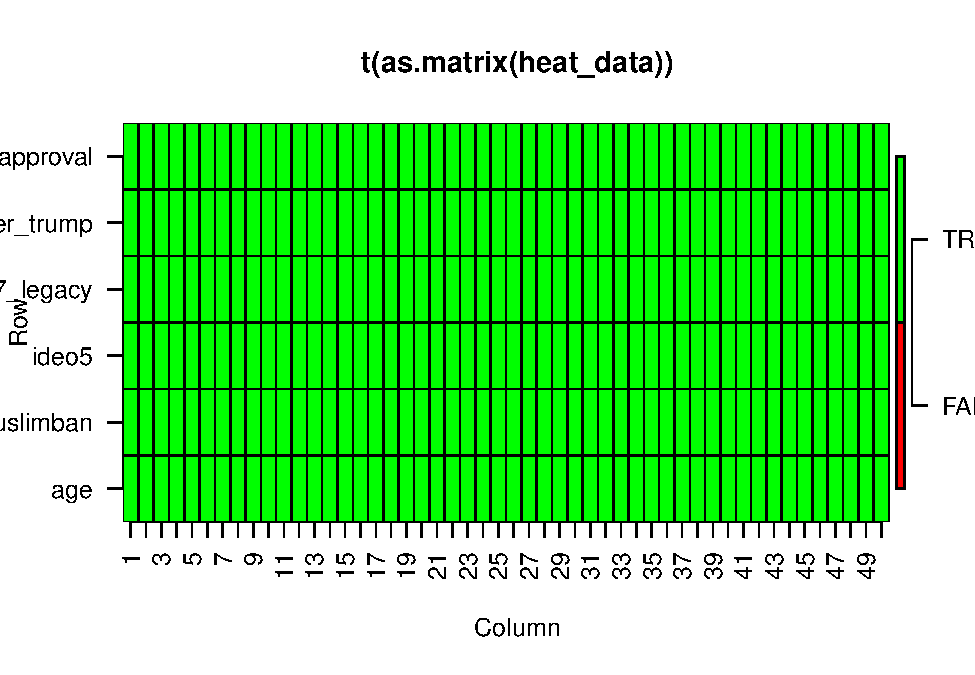
\includegraphics{data_assignment10_nov_11_2021_files/figure-latex/q2-1.pdf}

All data are present!

\hypertarget{question-3}{%
\subsection{Question 3}\label{question-3}}

\textbf{Based on what you have thought about and the data you have
found, clearly state a specific research question and a hypothesis.
Which channel (or channels) through which situational factors can affect
political behavior does your hypothesis implicate? (In class, we talked
about rational choice, priming, and emotional channels.)} The research
question should not be obvious ahead of time (although you should have a
theoretical expectation or competing hypotheses); it should be be
descriptive, correlational, or causal in nature; and it should be
answerable with the data you have available. Make sure your research
question is specific; don't confuse the research question with a
broader, motivating question that might be used to get people interested
in your topic.

My research question is "Did the first impeachment of Donald Trump cause
changes in people's political attitudes, policy positions, electoral
intentions, or ideology? And were these effects different for those who
were old enough to witness Bill Clinton's impeachment? This is an
example of how situational context could influence political behavior
through priming.

\hypertarget{question-4}{%
\subsection{Question 4}\label{question-4}}

In academic and professional settings, peer feedback, especially early
in a project, can force you to clarify your thinking and be an important
source of ideas. It's also important to be able to give a quick
`elevator pitch' for your project (so named because it can be delivered
in no more time than an elevator ride). We've randomly assigned you into
groups to share your ideas so far and get your peers' input about
sources you should read, different ways to approach your analysis, or
questions about your hypotheses. \textbf{Get together in your groups,
have everyone give their project's `elevator pitch,' and gather feedback
from your peers. Write at least one thing you took away from this
session.} The next couple of questions will ask you to try to use the
data to answer your research question and test your hypotheses, so be
sure to brainstorm good ways to approach those tasks.

Someone had the idea to include ``policy positions'' as well, so I added
that to my research question.

\hypertarget{question-5}{%
\subsection{Question 5}\label{question-5}}

No research project exists in a vacuum. As you get ready for your final
projects, we want you to practice finding, summarizing, and citing
related literature. \textbf{Identify at least two academic articles that
might provide some background for your research question. List the
complete source citations and include links to the articles you found.}
Google Scholar (\url{https://scholar.google.com/}) or Hollis
(\url{https://hollis.harvard.edu/}) are good places to look for these.

Jacobson, Gary C. ``Donald Trump and the parties: Impeachment, pandemic,
protest, and electoral politics in 2020.'' Presidential Studies
Quarterly 50.4 (2020): 762-795.
\href{https://onlinelibrary.wiley.com/doi/epdf/10.1111/psq.12682}{Link}

Lee, Changjun, Jieun Shin, and Ahreum Hong. ``Does social media use
really make people politically polarized? Direct and indirect effects of
social media use on political polarization in South Korea.'' Telematics
and Informatics 35.1 (2018): 245-254.
\href{https://www.sciencedirect.com/science/article/abs/pii/S0736585317305208}{Link}

\hypertarget{question-6}{%
\subsection{Question 6}\label{question-6}}

\textbf{Read in the data from the weeks surrounding your event of
interest and test your hypothesis. This can be something straightforward
like a difference-in-means or you can plot a visualization of the data.
Just take one of the approaches we have used in class before to get an
initial sense for if the data provide evidence of the contextual effects
you theorized.} Note that you might have to do a fair bit of data
cleaning in order to do this. Pay particular attention to how missing
data are coded.

\hypertarget{example}{%
\subsubsection{Example}\label{example}}

First we will need to load and compile the data for the several weeks
surrounding the mass shootings we are investigating.

\begin{Shaded}
\begin{Highlighting}[]
\CommentTok{# load the weekly survey files}

\NormalTok{Jul18 <-}\StringTok{ }\KeywordTok{read_dta}\NormalTok{(}\StringTok{'Nationscape-DataRelease_WeeklyMaterials_DTA/phase_1_v20200814/ns20191205/ns20191205.dta'}\NormalTok{) }\OperatorTok
\StringTok{  }\KeywordTok{remove_all_labels}\NormalTok{()}
\NormalTok{Jul25 <-}\StringTok{ }\KeywordTok{read_dta}\NormalTok{(}\StringTok{'Nationscape-dataRelease_WeeklyMaterials_DTA/phase_1_v20200814/ns20191212/ns20191212.dta'}\NormalTok{)}\OperatorTok
\StringTok{  }\KeywordTok{remove_all_labels}\NormalTok{()}
\NormalTok{Aug01 <-}\StringTok{ }\KeywordTok{read_dta}\NormalTok{(}\StringTok{'Nationscape-dataRelease_WeeklyMaterials_DTA/phase_1_v20200814/ns20191219/ns20191219.dta'}\NormalTok{) }\OperatorTok
\StringTok{  }\KeywordTok{remove_all_labels}\NormalTok{()}
\NormalTok{Aug08 <-}\StringTok{ }\KeywordTok{read_dta}\NormalTok{(}\StringTok{'Nationscape-dataRelease_WeeklyMaterials_DTA/phase_1_v20200814/ns20191226/ns20191226.dta'}\NormalTok{)}\OperatorTok
\StringTok{  }\KeywordTok{remove_all_labels}\NormalTok{()}
\NormalTok{Aug15 <-}\StringTok{ }\KeywordTok{read_dta}\NormalTok{(}\StringTok{'Nationscape-DataRelease_WeeklyMaterials_DTA/phase_2_v20200814/ns20200102/ns20200102.dta'}\NormalTok{)}\OperatorTok
\StringTok{  }\KeywordTok{remove_all_labels}\NormalTok{()}


\CommentTok{# join them all together}
\NormalTok{full_data <-}\StringTok{ }\KeywordTok{full_join}\NormalTok{(Jul18,Jul25) }\OperatorTok\StringTok{ }
\StringTok{  }\KeywordTok{full_join}\NormalTok{(., Aug01) }\OperatorTok
\StringTok{  }\KeywordTok{full_join}\NormalTok{(., Aug08) }\OperatorTok
\StringTok{  }\KeywordTok{full_join}\NormalTok{(., Aug15)}
\end{Highlighting}
\end{Shaded}

\begin{verbatim}
## Joining, by = c("response_id", "start_date", "right_track", "economy_better", "interest", "registration", "news_sources_facebook", "news_sources_cnn", "news_sources_msnbc", "news_sources_fox", "news_sources_network", "news_sources_localtv", "news_sources_telemundo", "news_sources_npr", "news_sources_amtalk", "news_sources_new_york_times", "news_sources_local_newspaper", "news_sources_other", "news_sources_other_TEXT", "pres_approval", "vote_intention", "vote_2016", "vote_2016_other_text", "consider_trump", "not_trump", "primary_party", "group_favorability_whites", "group_favorability_blacks", "group_favorability_latinos", "group_favorability_asians", "group_favorability_evangelicals", "group_favorability_socialists", "group_favorability_muslims", "group_favorability_labor_unions", "group_favorability_the_police", "group_favorability_undocumented", "group_favorability_lgbt", "group_favorability_republicans", "group_favorability_democrats", "group_favorability_white_men", "cand_favorability_trump", "cand_favorability_obama", "cand_favorability_biden", "cand_favorability_buttigieg", "cand_favorability_warren", "cand_favorability_sanders", "dem_vote_intent", "rank_dems_1", "rank_dems_2", "rank_dems_3", "rep_vote_prim", "rep_vote_prim_TEXT", "replace_trump", "house_intent", "senate_intent", "governor_intent", "trump_biden", "trump_sanders", "trump_warren", "trump_buttigieg", "pence_biden", "pence_buttigieg", "pence_sanders", "pence_warren", "primary_sen_barrasso", "primary_sen_blackburn", "primary_sen_blunt", "primary_sen_cassidy", "primary_sen_collins", "primary_sen_cornyn", "primary_sen_cotton", "primary_sen_daines", "primary_sen_ernst", "primary_sen_gardner", "primary_sen_graham", "primary_sen_hoeven", "primary_sen_hydesmith", "primary_sen_inhofe", "primary_sen_lee", "primary_sen_mcconnell", "primary_sen_mcsally", "primary_sen_moorecapito", "primary_sen_moran", "primary_sen_perdue", "primary_sen_portman", "primary_sen_risch", "primary_sen_rounds", "primary_sen_rubio", "primary_sen_sasse", "primary_sen_shelby", "primary_sen_sullivan", "primary_sen_tillis", "primary_sen_toomey", "primary_sen_young", "primary_sen_boozman", "primary_sen_braun", "primary_sen_cramer", "primary_sen_crapo", "primary_sen_cruz", "primary_sen_fischer", "primary_sen_grassley", "primary_sen_hawley", "primary_sen_lankford", "primary_sen_murkowski", "primary_sen_neelykennedy", "primary_sen_paul", "primary_sen_romney", "primary_sen_scott_rick", "primary_sen_scott_tim", "primary_sen_thune", "primary_sen_wicker", "cand_truth_donald_trump", "cand_truth_elizabeth_warren", "cand_truth_joe_biden", "cand_truth_bernie_sanders", "cand_truth_pete_buttigieg", "cand_facts_donald_trump", "cand_facts_elizabeth_warren", "cand_facts_joe_biden", "cand_facts_bernie_sanders", "cand_facts_pete_buttigieg", "racial_attitudes_tryhard", "racial_attitudes_generations", "racial_attitudes_marry", "racial_attitudes_date", "gender_attitudes_maleboss", "gender_attitudes_logical", "gender_attitudes_opportunity", "gender_attitudes_complain", "discrimination_blacks", "discrimination_whites", "discrimination_muslims", "discrimination_christians", "discrimination_women", "discrimination_men", "sen_knowledge", "sc_knowledge", "pid3", "pid7_legacy", "strength_democrat", "strength_republican", "lean_independent", "ideo5", "employment", "employment_other_text", "foreign_born", "language", "religion", "religion_other_text", "is_evangelical", "orientation_group", "in_union", "household_gun_owner", "wall", "cap_carbon", "guns_bg", "mctaxes", "estate_tax", "raise_upper_tax", "college", "abortion_any_time", "abortion_never", "abortion_conditions", "late_term_abortion", "abolish_priv_insurance", "abortion_insurance", "abortion_waiting", "china_tariffs", "criminal_immigration", "environment", "guaranteed_jobs", "green_new_deal", "gun_registry", "immigration_insurance", "immigration_separation", "immigration_system", "immigration_wire", "impeach_trump", "israel", "marijuana", "maternityleave", "medicare_for_all", "military_size", "minwage", "muslimban", "oil_and_gas", "reparations", "right_to_work", "ten_commandments", "trade", "trans_military", "uctaxes2", "vouchers", "gov_insurance", "public_option", "health_subsidies", "path_to_citizenship", "dreamers", "deportation", "ban_guns", "ban_assault_rifles", "limit_magazines", "fc_smallgov", "fc_trad_val", "statements_protect_traditions", "statements_defense_burden", "statements_trade_effects", "statements_christianity_assault", "statements_gender_identity", "statements_american_loss", "statements_imm_assimilate", "statements_gun_rights", "statements_confront_china", "statements_foreign_interests", "extra_group_favor_demcong", "extra_group_favor_repcong", "age", "gender", "census_region", "hispanic", "race_ethnicity", "household_income", "education", "state", "congress_district", "weight")
\end{verbatim}

\begin{verbatim}
## Joining, by = c("response_id", "start_date", "right_track", "economy_better", "interest", "registration", "news_sources_facebook", "news_sources_cnn", "news_sources_msnbc", "news_sources_fox", "news_sources_network", "news_sources_localtv", "news_sources_telemundo", "news_sources_npr", "news_sources_amtalk", "news_sources_new_york_times", "news_sources_local_newspaper", "news_sources_other", "news_sources_other_TEXT", "pres_approval", "vote_intention", "vote_2016", "vote_2016_other_text", "consider_trump", "not_trump", "primary_party", "group_favorability_whites", "group_favorability_blacks", "group_favorability_latinos", "group_favorability_asians", "group_favorability_evangelicals", "group_favorability_socialists", "group_favorability_muslims", "group_favorability_labor_unions", "group_favorability_the_police", "group_favorability_undocumented", "group_favorability_lgbt", "group_favorability_republicans", "group_favorability_democrats", "group_favorability_white_men", "cand_favorability_trump", "cand_favorability_obama", "cand_favorability_biden", "cand_favorability_buttigieg", "cand_favorability_warren", "cand_favorability_sanders", "dem_vote_intent", "rank_dems_1", "rank_dems_2", "rank_dems_3", "rep_vote_prim", "rep_vote_prim_TEXT", "replace_trump", "house_intent", "senate_intent", "governor_intent", "trump_biden", "trump_sanders", "trump_warren", "trump_buttigieg", "pence_biden", "pence_buttigieg", "pence_sanders", "pence_warren", "primary_sen_barrasso", "primary_sen_blackburn", "primary_sen_blunt", "primary_sen_cassidy", "primary_sen_collins", "primary_sen_cornyn", "primary_sen_cotton", "primary_sen_daines", "primary_sen_ernst", "primary_sen_gardner", "primary_sen_graham", "primary_sen_hoeven", "primary_sen_hydesmith", "primary_sen_inhofe", "primary_sen_lee", "primary_sen_mcconnell", "primary_sen_mcsally", "primary_sen_moorecapito", "primary_sen_moran", "primary_sen_perdue", "primary_sen_portman", "primary_sen_risch", "primary_sen_rounds", "primary_sen_rubio", "primary_sen_sasse", "primary_sen_shelby", "primary_sen_sullivan", "primary_sen_tillis", "primary_sen_toomey", "primary_sen_young", "primary_sen_boozman", "primary_sen_braun", "primary_sen_cramer", "primary_sen_crapo", "primary_sen_cruz", "primary_sen_fischer", "primary_sen_grassley", "primary_sen_hawley", "primary_sen_lankford", "primary_sen_murkowski", "primary_sen_neelykennedy", "primary_sen_paul", "primary_sen_romney", "primary_sen_scott_rick", "primary_sen_scott_tim", "primary_sen_thune", "primary_sen_wicker", "cand_truth_donald_trump", "cand_truth_elizabeth_warren", "cand_truth_joe_biden", "cand_truth_bernie_sanders", "cand_truth_pete_buttigieg", "cand_facts_donald_trump", "cand_facts_elizabeth_warren", "cand_facts_joe_biden", "cand_facts_bernie_sanders", "cand_facts_pete_buttigieg", "racial_attitudes_tryhard", "racial_attitudes_generations", "racial_attitudes_marry", "racial_attitudes_date", "gender_attitudes_maleboss", "gender_attitudes_logical", "gender_attitudes_opportunity", "gender_attitudes_complain", "discrimination_blacks", "discrimination_whites", "discrimination_muslims", "discrimination_christians", "discrimination_women", "discrimination_men", "sen_knowledge", "sc_knowledge", "pid3", "pid7_legacy", "strength_democrat", "strength_republican", "lean_independent", "ideo5", "employment", "employment_other_text", "foreign_born", "language", "religion", "religion_other_text", "is_evangelical", "orientation_group", "in_union", "household_gun_owner", "wall", "cap_carbon", "guns_bg", "mctaxes", "estate_tax", "raise_upper_tax", "college", "abortion_any_time", "abortion_never", "abortion_conditions", "late_term_abortion", "abolish_priv_insurance", "abortion_insurance", "abortion_waiting", "china_tariffs", "criminal_immigration", "environment", "guaranteed_jobs", "green_new_deal", "gun_registry", "immigration_insurance", "immigration_separation", "immigration_system", "immigration_wire", "impeach_trump", "israel", "marijuana", "maternityleave", "medicare_for_all", "military_size", "minwage", "muslimban", "oil_and_gas", "reparations", "right_to_work", "ten_commandments", "trade", "trans_military", "uctaxes2", "vouchers", "gov_insurance", "public_option", "health_subsidies", "path_to_citizenship", "dreamers", "deportation", "ban_guns", "ban_assault_rifles", "limit_magazines", "fc_smallgov", "fc_trad_val", "statements_protect_traditions", "statements_defense_burden", "statements_trade_effects", "statements_christianity_assault", "statements_gender_identity", "statements_american_loss", "statements_imm_assimilate", "statements_gun_rights", "statements_confront_china", "statements_foreign_interests", "extra_group_favor_demcong", "extra_group_favor_repcong", "age", "gender", "census_region", "hispanic", "race_ethnicity", "household_income", "education", "state", "congress_district", "weight", "group_favorability_jews", "discrimination_jews")
## Joining, by = c("response_id", "start_date", "right_track", "economy_better", "interest", "registration", "news_sources_facebook", "news_sources_cnn", "news_sources_msnbc", "news_sources_fox", "news_sources_network", "news_sources_localtv", "news_sources_telemundo", "news_sources_npr", "news_sources_amtalk", "news_sources_new_york_times", "news_sources_local_newspaper", "news_sources_other", "news_sources_other_TEXT", "pres_approval", "vote_intention", "vote_2016", "vote_2016_other_text", "consider_trump", "not_trump", "primary_party", "group_favorability_whites", "group_favorability_blacks", "group_favorability_latinos", "group_favorability_asians", "group_favorability_evangelicals", "group_favorability_socialists", "group_favorability_muslims", "group_favorability_labor_unions", "group_favorability_the_police", "group_favorability_undocumented", "group_favorability_lgbt", "group_favorability_republicans", "group_favorability_democrats", "group_favorability_white_men", "cand_favorability_trump", "cand_favorability_obama", "cand_favorability_biden", "cand_favorability_buttigieg", "cand_favorability_warren", "cand_favorability_sanders", "dem_vote_intent", "rank_dems_1", "rank_dems_2", "rank_dems_3", "rep_vote_prim", "rep_vote_prim_TEXT", "replace_trump", "house_intent", "senate_intent", "governor_intent", "trump_biden", "trump_sanders", "trump_warren", "trump_buttigieg", "pence_biden", "pence_buttigieg", "pence_sanders", "pence_warren", "primary_sen_barrasso", "primary_sen_blackburn", "primary_sen_blunt", "primary_sen_cassidy", "primary_sen_collins", "primary_sen_cornyn", "primary_sen_cotton", "primary_sen_daines", "primary_sen_ernst", "primary_sen_gardner", "primary_sen_graham", "primary_sen_hoeven", "primary_sen_hydesmith", "primary_sen_inhofe", "primary_sen_lee", "primary_sen_mcconnell", "primary_sen_mcsally", "primary_sen_moorecapito", "primary_sen_moran", "primary_sen_perdue", "primary_sen_portman", "primary_sen_risch", "primary_sen_rounds", "primary_sen_rubio", "primary_sen_sasse", "primary_sen_shelby", "primary_sen_sullivan", "primary_sen_tillis", "primary_sen_toomey", "primary_sen_young", "primary_sen_boozman", "primary_sen_braun", "primary_sen_cramer", "primary_sen_crapo", "primary_sen_cruz", "primary_sen_fischer", "primary_sen_grassley", "primary_sen_hawley", "primary_sen_lankford", "primary_sen_murkowski", "primary_sen_neelykennedy", "primary_sen_paul", "primary_sen_romney", "primary_sen_scott_rick", "primary_sen_scott_tim", "primary_sen_thune", "primary_sen_wicker", "cand_truth_donald_trump", "cand_truth_elizabeth_warren", "cand_truth_joe_biden", "cand_truth_bernie_sanders", "cand_truth_pete_buttigieg", "cand_facts_donald_trump", "cand_facts_elizabeth_warren", "cand_facts_joe_biden", "cand_facts_bernie_sanders", "cand_facts_pete_buttigieg", "racial_attitudes_tryhard", "racial_attitudes_generations", "racial_attitudes_marry", "racial_attitudes_date", "gender_attitudes_maleboss", "gender_attitudes_logical", "gender_attitudes_opportunity", "gender_attitudes_complain", "discrimination_blacks", "discrimination_whites", "discrimination_muslims", "discrimination_christians", "discrimination_women", "discrimination_men", "sen_knowledge", "sc_knowledge", "pid3", "pid7_legacy", "strength_democrat", "strength_republican", "lean_independent", "ideo5", "employment", "employment_other_text", "foreign_born", "language", "religion", "religion_other_text", "is_evangelical", "orientation_group", "in_union", "household_gun_owner", "wall", "cap_carbon", "guns_bg", "mctaxes", "estate_tax", "raise_upper_tax", "college", "abortion_any_time", "abortion_never", "abortion_conditions", "late_term_abortion", "abolish_priv_insurance", "abortion_insurance", "abortion_waiting", "china_tariffs", "criminal_immigration", "environment", "guaranteed_jobs", "green_new_deal", "gun_registry", "immigration_insurance", "immigration_separation", "immigration_system", "immigration_wire", "impeach_trump", "israel", "marijuana", "maternityleave", "medicare_for_all", "military_size", "minwage", "muslimban", "oil_and_gas", "reparations", "right_to_work", "ten_commandments", "trade", "trans_military", "uctaxes2", "vouchers", "gov_insurance", "public_option", "health_subsidies", "path_to_citizenship", "dreamers", "deportation", "ban_guns", "ban_assault_rifles", "limit_magazines", "fc_smallgov", "fc_trad_val", "statements_protect_traditions", "statements_defense_burden", "statements_trade_effects", "statements_christianity_assault", "statements_gender_identity", "statements_american_loss", "statements_imm_assimilate", "statements_gun_rights", "statements_confront_china", "statements_foreign_interests", "extra_group_favor_demcong", "extra_group_favor_repcong", "age", "gender", "census_region", "hispanic", "race_ethnicity", "household_income", "education", "state", "congress_district", "weight", "group_favorability_jews", "discrimination_jews")
\end{verbatim}

\begin{verbatim}
## Joining, by = c("response_id", "start_date", "right_track", "economy_better", "interest", "registration", "news_sources_facebook", "news_sources_cnn", "news_sources_msnbc", "news_sources_fox", "news_sources_network", "news_sources_localtv", "news_sources_telemundo", "news_sources_npr", "news_sources_amtalk", "news_sources_new_york_times", "news_sources_local_newspaper", "news_sources_other", "news_sources_other_TEXT", "pres_approval", "vote_intention", "vote_2016", "vote_2016_other_text", "consider_trump", "not_trump", "primary_party", "group_favorability_whites", "group_favorability_blacks", "group_favorability_latinos", "group_favorability_asians", "group_favorability_evangelicals", "group_favorability_socialists", "group_favorability_muslims", "group_favorability_labor_unions", "group_favorability_the_police", "group_favorability_undocumented", "group_favorability_lgbt", "group_favorability_republicans", "group_favorability_democrats", "group_favorability_white_men", "cand_favorability_trump", "cand_favorability_obama", "cand_favorability_biden", "cand_favorability_buttigieg", "cand_favorability_warren", "cand_favorability_sanders", "dem_vote_intent", "rank_dems_1", "rank_dems_2", "rank_dems_3", "rep_vote_prim", "rep_vote_prim_TEXT", "replace_trump", "house_intent", "senate_intent", "governor_intent", "trump_biden", "trump_sanders", "trump_warren", "trump_buttigieg", "pence_biden", "pence_buttigieg", "pence_sanders", "pence_warren", "primary_sen_barrasso", "primary_sen_blackburn", "primary_sen_blunt", "primary_sen_cassidy", "primary_sen_collins", "primary_sen_cornyn", "primary_sen_cotton", "primary_sen_daines", "primary_sen_ernst", "primary_sen_gardner", "primary_sen_graham", "primary_sen_hoeven", "primary_sen_hydesmith", "primary_sen_inhofe", "primary_sen_lee", "primary_sen_mcconnell", "primary_sen_mcsally", "primary_sen_moorecapito", "primary_sen_moran", "primary_sen_perdue", "primary_sen_portman", "primary_sen_risch", "primary_sen_rounds", "primary_sen_rubio", "primary_sen_sasse", "primary_sen_shelby", "primary_sen_sullivan", "primary_sen_tillis", "primary_sen_toomey", "primary_sen_young", "primary_sen_boozman", "primary_sen_braun", "primary_sen_cramer", "primary_sen_crapo", "primary_sen_cruz", "primary_sen_fischer", "primary_sen_grassley", "primary_sen_hawley", "primary_sen_lankford", "primary_sen_murkowski", "primary_sen_neelykennedy", "primary_sen_paul", "primary_sen_romney", "primary_sen_scott_rick", "primary_sen_scott_tim", "primary_sen_thune", "primary_sen_wicker", "cand_truth_donald_trump", "cand_truth_elizabeth_warren", "cand_truth_joe_biden", "cand_truth_bernie_sanders", "cand_truth_pete_buttigieg", "cand_facts_donald_trump", "cand_facts_elizabeth_warren", "cand_facts_joe_biden", "cand_facts_bernie_sanders", "cand_facts_pete_buttigieg", "racial_attitudes_tryhard", "racial_attitudes_generations", "racial_attitudes_marry", "racial_attitudes_date", "gender_attitudes_maleboss", "gender_attitudes_logical", "gender_attitudes_opportunity", "gender_attitudes_complain", "discrimination_blacks", "discrimination_whites", "discrimination_muslims", "discrimination_christians", "discrimination_women", "discrimination_men", "sen_knowledge", "sc_knowledge", "pid3", "pid7_legacy", "strength_democrat", "strength_republican", "lean_independent", "ideo5", "employment", "employment_other_text", "foreign_born", "language", "religion", "religion_other_text", "is_evangelical", "orientation_group", "in_union", "household_gun_owner", "wall", "cap_carbon", "guns_bg", "mctaxes", "estate_tax", "raise_upper_tax", "college", "abortion_any_time", "abortion_never", "abortion_conditions", "late_term_abortion", "abolish_priv_insurance", "abortion_insurance", "abortion_waiting", "china_tariffs", "criminal_immigration", "environment", "guaranteed_jobs", "green_new_deal", "gun_registry", "immigration_insurance", "immigration_separation", "immigration_system", "immigration_wire", "impeach_trump", "israel", "marijuana", "maternityleave", "medicare_for_all", "military_size", "minwage", "muslimban", "oil_and_gas", "reparations", "right_to_work", "ten_commandments", "trade", "trans_military", "uctaxes2", "vouchers", "gov_insurance", "public_option", "health_subsidies", "path_to_citizenship", "dreamers", "deportation", "ban_guns", "ban_assault_rifles", "limit_magazines", "fc_smallgov", "fc_trad_val", "statements_protect_traditions", "statements_defense_burden", "statements_trade_effects", "statements_christianity_assault", "statements_gender_identity", "statements_american_loss", "statements_imm_assimilate", "statements_gun_rights", "statements_confront_china", "statements_foreign_interests", "extra_group_favor_demcong", "extra_group_favor_repcong", "age", "gender", "census_region", "hispanic", "race_ethnicity", "household_income", "education", "state", "congress_district", "weight", "group_favorability_jews", "discrimination_jews", "extra_party_ideo_rate_dem", "extra_party_ideo_rate_rep", "extra_party_ideo_dem_desire", "extra_party_ideo_rep_desire")
\end{verbatim}

\begin{Shaded}
\begin{Highlighting}[]
\CommentTok{# recode NAs}
\NormalTok{full_data <-}\StringTok{ }\NormalTok{full_data }\OperatorTok
\StringTok{  }\KeywordTok{mutate}\NormalTok{(}\KeywordTok{across}\NormalTok{(}\DataTypeTok{.cols =} \KeywordTok{everything}\NormalTok{(), }\OperatorTok{~}\KeywordTok{na_if}\NormalTok{(., }\DecValTok{999}\NormalTok{))) }\OperatorTok
\StringTok{  }\KeywordTok{mutate}\NormalTok{(}\KeywordTok{across}\NormalTok{(}\DataTypeTok{.cols =} \KeywordTok{everything}\NormalTok{(), }\OperatorTok{~}\KeywordTok{na_if}\NormalTok{(., }\DecValTok{888}\NormalTok{)))}
\end{Highlighting}
\end{Shaded}

\begin{Shaded}
\begin{Highlighting}[]
\CommentTok{# create an indicator variable for surveys administered after impeachment}
\NormalTok{full_data <-}\StringTok{ }\NormalTok{full_data }\OperatorTok
\StringTok{  }\KeywordTok{mutate}\NormalTok{(}\DataTypeTok{treated =} \KeywordTok{if_else}\NormalTok{(start_date }\OperatorTok{>}\StringTok{ }\KeywordTok{as.Date}\NormalTok{(}\StringTok{'2019-12-18'}\NormalTok{), }\OtherTok{TRUE}\NormalTok{, }\OtherTok{FALSE}\NormalTok{)) }\OperatorTok\StringTok{ }
\StringTok{  }\KeywordTok{mutate}\NormalTok{(}\DataTypeTok{witnessed_bc_imp =} \KeywordTok{if_else}\NormalTok{(age }\OperatorTok{>}\StringTok{ }\DecValTok{39}\NormalTok{, }\OtherTok{TRUE}\NormalTok{, }\OtherTok{FALSE}\NormalTok{)) }\OperatorTok
\StringTok{  }\KeywordTok{select}\NormalTok{(start_date, pres_approval, consider_trump, pid7_legacy, ideo5, muslimban, age, treated, witnessed_bc_imp)}
\end{Highlighting}
\end{Shaded}

As a first cut, we can try a difference in means. Don't forget to check
the effect size.

\begin{Shaded}
\begin{Highlighting}[]
\KeywordTok{difference_in_means}\NormalTok{(pres_approval }\OperatorTok{~}\StringTok{ }\NormalTok{treated, }\DataTypeTok{data =}\NormalTok{ full_data }\OperatorTok\StringTok{ }\KeywordTok{filter}\NormalTok{(}\KeywordTok{as.Date}\NormalTok{(}\StringTok{'2019-12-05'}\NormalTok{) }\OperatorTok{<}\StringTok{ }\NormalTok{start_date) }\OperatorTok\StringTok{ }\KeywordTok{filter}\NormalTok{(start_date }\OperatorTok{<}\StringTok{ }\KeywordTok{as.Date}\NormalTok{(}\StringTok{'2020-01-02'}\NormalTok{)))}
\end{Highlighting}
\end{Shaded}

\begin{verbatim}
## Design:  Standard 
##           Estimate Std. Error  t value  Pr(>|t|)     CI Lower   CI Upper
## treated 0.02142385 0.01535049 1.395646 0.1628337 -0.008664046 0.05151175
##               DF
## treated 24343.78
\end{verbatim}

\begin{Shaded}
\begin{Highlighting}[]
\KeywordTok{difference_in_means}\NormalTok{(consider_trump }\OperatorTok{~}\StringTok{ }\NormalTok{treated, }\DataTypeTok{data =}\NormalTok{ full_data }\OperatorTok\StringTok{ }\KeywordTok{filter}\NormalTok{(}\KeywordTok{as.Date}\NormalTok{(}\StringTok{'2019-12-05'}\NormalTok{) }\OperatorTok{<}\StringTok{ }\NormalTok{start_date) }\OperatorTok\StringTok{ }\KeywordTok{filter}\NormalTok{(start_date }\OperatorTok{<}\StringTok{ }\KeywordTok{as.Date}\NormalTok{(}\StringTok{'2020-01-02'}\NormalTok{)))}
\end{Highlighting}
\end{Shaded}

\begin{verbatim}
## Design:  Standard 
##            Estimate  Std. Error   t value  Pr(>|t|)    CI Lower   CI Upper
## treated 0.004322577 0.006344273 0.6813354 0.4956662 -0.00811263 0.01675778
##               DF
## treated 22780.57
\end{verbatim}

\begin{Shaded}
\begin{Highlighting}[]
\KeywordTok{difference_in_means}\NormalTok{(pid7_legacy }\OperatorTok{~}\StringTok{ }\NormalTok{treated, }\DataTypeTok{data =}\NormalTok{ full_data }\OperatorTok\StringTok{ }\KeywordTok{filter}\NormalTok{(}\KeywordTok{as.Date}\NormalTok{(}\StringTok{'2019-12-05'}\NormalTok{) }\OperatorTok{<}\StringTok{ }\NormalTok{start_date) }\OperatorTok\StringTok{ }\KeywordTok{filter}\NormalTok{(start_date }\OperatorTok{<}\StringTok{ }\KeywordTok{as.Date}\NormalTok{(}\StringTok{'2020-01-02'}\NormalTok{)))}
\end{Highlighting}
\end{Shaded}

\begin{verbatim}
## Design:  Standard 
##            Estimate Std. Error   t value    Pr(>|t|)   CI Lower    CI Upper
## treated -0.08393713 0.02839435 -2.956121 0.003118424 -0.1395919 -0.02828238
##               DF
## treated 23638.96
\end{verbatim}

\begin{Shaded}
\begin{Highlighting}[]
\KeywordTok{difference_in_means}\NormalTok{(ideo5 }\OperatorTok{~}\StringTok{ }\NormalTok{treated, }\DataTypeTok{data =}\NormalTok{ full_data }\OperatorTok\StringTok{ }\KeywordTok{filter}\NormalTok{(}\KeywordTok{as.Date}\NormalTok{(}\StringTok{'2019-12-05'}\NormalTok{) }\OperatorTok{<}\StringTok{ }\NormalTok{start_date) }\OperatorTok\StringTok{ }\KeywordTok{filter}\NormalTok{(start_date }\OperatorTok{<}\StringTok{ }\KeywordTok{as.Date}\NormalTok{(}\StringTok{'2020-01-02'}\NormalTok{)))}
\end{Highlighting}
\end{Shaded}

\begin{verbatim}
## Design:  Standard 
##            Estimate Std. Error   t value   Pr(>|t|)    CI Lower    CI Upper
## treated -0.03937721 0.01490641 -2.641629 0.00825664 -0.06859484 -0.01015958
##               DF
## treated 22092.19
\end{verbatim}

\begin{Shaded}
\begin{Highlighting}[]
\KeywordTok{difference_in_means}\NormalTok{(muslimban }\OperatorTok{~}\StringTok{ }\NormalTok{treated, }\DataTypeTok{data =}\NormalTok{ full_data }\OperatorTok\StringTok{ }\KeywordTok{filter}\NormalTok{(}\KeywordTok{as.Date}\NormalTok{(}\StringTok{'2019-12-05'}\NormalTok{) }\OperatorTok{<}\StringTok{ }\NormalTok{start_date) }\OperatorTok\StringTok{ }\KeywordTok{filter}\NormalTok{(start_date }\OperatorTok{<}\StringTok{ }\KeywordTok{as.Date}\NormalTok{(}\StringTok{'2020-01-02'}\NormalTok{)))}
\end{Highlighting}
\end{Shaded}

\begin{verbatim}
## Design:  Standard 
##           Estimate Std. Error  t value   Pr(>|t|)      CI Lower   CI Upper
## treated 0.02125276 0.01132051 1.877368 0.06051542 -0.0009394378 0.04344496
##               DF
## treated 6097.761
\end{verbatim}

\begin{Shaded}
\begin{Highlighting}[]
\KeywordTok{difference_in_means}\NormalTok{(witnessed_bc_imp }\OperatorTok{~}\StringTok{ }\NormalTok{treated, }\DataTypeTok{data =}\NormalTok{ full_data }\OperatorTok\StringTok{ }\KeywordTok{filter}\NormalTok{(}\KeywordTok{as.Date}\NormalTok{(}\StringTok{'2019-12-05'}\NormalTok{) }\OperatorTok{<}\StringTok{ }\NormalTok{start_date) }\OperatorTok\StringTok{ }\KeywordTok{filter}\NormalTok{(start_date }\OperatorTok{<}\StringTok{ }\KeywordTok{as.Date}\NormalTok{(}\StringTok{'2020-01-02'}\NormalTok{)))}
\end{Highlighting}
\end{Shaded}

\begin{verbatim}
## Design:  Standard 
##           Estimate  Std. Error t value     Pr(>|t|)    CI Lower   CI Upper
## treated 0.02077763 0.006062797 3.42707 0.0006111003 0.008894197 0.03266106
##               DF
## treated 25359.43
\end{verbatim}

\begin{Shaded}
\begin{Highlighting}[]
\KeywordTok{difference_in_means}\NormalTok{(age }\OperatorTok{~}\StringTok{ }\NormalTok{treated, }\DataTypeTok{data =}\NormalTok{ full_data }\OperatorTok\StringTok{ }\KeywordTok{filter}\NormalTok{(}\KeywordTok{as.Date}\NormalTok{(}\StringTok{'2019-12-05'}\NormalTok{) }\OperatorTok{<}\StringTok{ }\NormalTok{start_date) }\OperatorTok\StringTok{ }\KeywordTok{filter}\NormalTok{(start_date }\OperatorTok{<}\StringTok{ }\KeywordTok{as.Date}\NormalTok{(}\StringTok{'2020-01-02'}\NormalTok{)))}
\end{Highlighting}
\end{Shaded}

\begin{verbatim}
## Design:  Standard 
##          Estimate Std. Error  t value   Pr(>|t|)   CI Lower  CI Upper       DF
## treated 0.4735844  0.2058072 2.301107 0.02139368 0.07019036 0.8769785 25306.12
\end{verbatim}

In order of greatest to least effect on the treatment: party preference,
ideology, presidential approval, view on the muslim ban, witnessed Bill
Clinton's impeachment, and consideration of Trump for 2020.

\begin{Shaded}
\begin{Highlighting}[]
\NormalTok{pres_approval_graph <-}\StringTok{ }\NormalTok{full_data }\OperatorTok
\StringTok{  }\KeywordTok{mutate}\NormalTok{(}\DataTypeTok{date =} \KeywordTok{as.Date}\NormalTok{(start_date)) }\OperatorTok
\StringTok{  }\KeywordTok{group_by}\NormalTok{(date) }\OperatorTok
\StringTok{  }\KeywordTok{summarize}\NormalTok{(}\DataTypeTok{pres_approval =} \KeywordTok{mean}\NormalTok{(pres_approval, }\DataTypeTok{na.rm =} \OtherTok{TRUE}\NormalTok{)) }\OperatorTok
\StringTok{  }\KeywordTok{ggplot}\NormalTok{(}\KeywordTok{aes}\NormalTok{(}\DataTypeTok{x =}\NormalTok{ date, }\DataTypeTok{y =}\NormalTok{ pres_approval)) }\OperatorTok{+}
\StringTok{  }\KeywordTok{geom_line}\NormalTok{() }\OperatorTok{+}
\StringTok{  }\KeywordTok{geom_vline}\NormalTok{(}\DataTypeTok{xintercept =} \KeywordTok{as.Date}\NormalTok{(}\StringTok{"2019-12-18"}\NormalTok{), }\DataTypeTok{color =} \StringTok{"red"}\NormalTok{) }\OperatorTok{+}
\StringTok{  }\KeywordTok{labs}\NormalTok{(}\DataTypeTok{title =} \StringTok{"Presidential Dispproval Before and After 12-18 Impeachment Vote"}\NormalTok{, }\DataTypeTok{subtitle =} \StringTok{"Higher Scores Mean Less Approval"}\NormalTok{) }\OperatorTok{+}
\StringTok{  }\KeywordTok{annotate}\NormalTok{(}\StringTok{"text"}\NormalTok{, }\DataTypeTok{x  =} \KeywordTok{as.Date}\NormalTok{(}\StringTok{"2019-12-30"}\NormalTok{), }\DataTypeTok{y=}\FloatTok{2.55}\NormalTok{, }\DataTypeTok{label =} \KeywordTok{paste}\NormalTok{(}\StringTok{"diff. in means before/after: "}\NormalTok{, (}\KeywordTok{difference_in_means}\NormalTok{(pres_approval }\OperatorTok{~}\StringTok{ }\NormalTok{treated, }\DataTypeTok{data =}\NormalTok{ full_data }\OperatorTok\StringTok{ }\KeywordTok{filter}\NormalTok{(}\KeywordTok{as.Date}\NormalTok{(}\StringTok{'2019-12-05'}\NormalTok{) }\OperatorTok{<}\StringTok{ }\NormalTok{start_date) }\OperatorTok\StringTok{ }\KeywordTok{filter}\NormalTok{(start_date }\OperatorTok{<}\StringTok{ }\KeywordTok{as.Date}\NormalTok{(}\StringTok{'2020-01-02'}\NormalTok{)))}\OperatorTok{$}\NormalTok{coefficient[[}\DecValTok{1}\NormalTok{]])))}

\NormalTok{consider_trump_graph <-}\StringTok{ }\NormalTok{full_data }\OperatorTok
\StringTok{  }\KeywordTok{mutate}\NormalTok{(}\DataTypeTok{date =} \KeywordTok{as.Date}\NormalTok{(start_date)) }\OperatorTok
\StringTok{  }\KeywordTok{group_by}\NormalTok{(date) }\OperatorTok
\StringTok{  }\KeywordTok{summarize}\NormalTok{(}\DataTypeTok{consider_trump =} \KeywordTok{mean}\NormalTok{(consider_trump, }\DataTypeTok{na.rm =} \OtherTok{TRUE}\NormalTok{)) }\OperatorTok
\StringTok{  }\KeywordTok{ggplot}\NormalTok{(}\KeywordTok{aes}\NormalTok{(}\DataTypeTok{x =}\NormalTok{ date, }\DataTypeTok{y =}\NormalTok{ consider_trump)) }\OperatorTok{+}
\StringTok{  }\KeywordTok{geom_line}\NormalTok{() }\OperatorTok{+}
\StringTok{  }\KeywordTok{geom_vline}\NormalTok{(}\DataTypeTok{xintercept =} \KeywordTok{as.Date}\NormalTok{(}\StringTok{"2019-12-18"}\NormalTok{), }\DataTypeTok{color =} \StringTok{"red"}\NormalTok{) }\OperatorTok{+}
\StringTok{  }\KeywordTok{labs}\NormalTok{(}\DataTypeTok{title =} \StringTok{"Consideration of Trump for 2020 Election Before and After 12-18 Impeachment Vote"}\NormalTok{, }\DataTypeTok{subtitle =} \StringTok{"Higher Scores Mean Less Consideration"}\NormalTok{) }\OperatorTok{+}
\StringTok{  }\KeywordTok{annotate}\NormalTok{(}\StringTok{"text"}\NormalTok{, }\DataTypeTok{x  =} \KeywordTok{as.Date}\NormalTok{(}\StringTok{"2019-12-30"}\NormalTok{), }\DataTypeTok{y=}\FloatTok{1.53}\NormalTok{, }\DataTypeTok{label =} \KeywordTok{paste}\NormalTok{(}\StringTok{"diff. in means before/after: "}\NormalTok{, (}\KeywordTok{difference_in_means}\NormalTok{(consider_trump }\OperatorTok{~}\StringTok{ }\NormalTok{treated, }\DataTypeTok{data =}\NormalTok{ full_data }\OperatorTok\StringTok{ }\KeywordTok{filter}\NormalTok{(}\KeywordTok{as.Date}\NormalTok{(}\StringTok{'2019-12-05'}\NormalTok{) }\OperatorTok{<}\StringTok{ }\NormalTok{start_date) }\OperatorTok\StringTok{ }\KeywordTok{filter}\NormalTok{(start_date }\OperatorTok{<}\StringTok{ }\KeywordTok{as.Date}\NormalTok{(}\StringTok{'2020-01-02'}\NormalTok{)))}\OperatorTok{$}\NormalTok{coefficient[[}\DecValTok{1}\NormalTok{]])))}

\NormalTok{pid7_legacy_graph <-}\StringTok{ }\NormalTok{full_data }\OperatorTok
\StringTok{  }\KeywordTok{mutate}\NormalTok{(}\DataTypeTok{date =} \KeywordTok{as.Date}\NormalTok{(start_date)) }\OperatorTok
\StringTok{  }\KeywordTok{group_by}\NormalTok{(date) }\OperatorTok
\StringTok{  }\KeywordTok{summarize}\NormalTok{(}\DataTypeTok{pid7_legacy =} \KeywordTok{mean}\NormalTok{(pid7_legacy, }\DataTypeTok{na.rm =} \OtherTok{TRUE}\NormalTok{)) }\OperatorTok
\StringTok{  }\KeywordTok{ggplot}\NormalTok{(}\KeywordTok{aes}\NormalTok{(}\DataTypeTok{x =}\NormalTok{ date, }\DataTypeTok{y =}\NormalTok{ pid7_legacy)) }\OperatorTok{+}
\StringTok{  }\KeywordTok{geom_line}\NormalTok{() }\OperatorTok{+}
\StringTok{  }\KeywordTok{geom_vline}\NormalTok{(}\DataTypeTok{xintercept =} \KeywordTok{as.Date}\NormalTok{(}\StringTok{"2019-12-18"}\NormalTok{), }\DataTypeTok{color =} \StringTok{"red"}\NormalTok{) }\OperatorTok{+}
\StringTok{  }\KeywordTok{labs}\NormalTok{(}\DataTypeTok{title =} \StringTok{"Party Identification Before and After 12-18 Impeachment Vote"}\NormalTok{, }\DataTypeTok{subtitle =} \StringTok{"1 = Strong D, 7 = Strong R"}\NormalTok{)  }\OperatorTok{+}
\StringTok{  }\KeywordTok{annotate}\NormalTok{(}\StringTok{"text"}\NormalTok{, }\DataTypeTok{x  =} \KeywordTok{as.Date}\NormalTok{(}\StringTok{"2019-12-30"}\NormalTok{), }\DataTypeTok{y=}\FloatTok{4.2}\NormalTok{, }\DataTypeTok{label =} \KeywordTok{paste}\NormalTok{(}\StringTok{"diff. in means before/after: "}\NormalTok{, (}\KeywordTok{difference_in_means}\NormalTok{(pid7_legacy }\OperatorTok{~}\StringTok{ }\NormalTok{treated, }\DataTypeTok{data =}\NormalTok{ full_data }\OperatorTok\StringTok{ }\KeywordTok{filter}\NormalTok{(}\KeywordTok{as.Date}\NormalTok{(}\StringTok{'2019-12-05'}\NormalTok{) }\OperatorTok{<}\StringTok{ }\NormalTok{start_date) }\OperatorTok\StringTok{ }\KeywordTok{filter}\NormalTok{(start_date }\OperatorTok{<}\StringTok{ }\KeywordTok{as.Date}\NormalTok{(}\StringTok{'2020-01-02'}\NormalTok{)))}\OperatorTok{$}\NormalTok{coefficient[[}\DecValTok{1}\NormalTok{]])))}

\NormalTok{ideo5_graph <-}\StringTok{ }\NormalTok{full_data }\OperatorTok
\StringTok{  }\KeywordTok{mutate}\NormalTok{(}\DataTypeTok{date =} \KeywordTok{as.Date}\NormalTok{(start_date)) }\OperatorTok
\StringTok{  }\KeywordTok{group_by}\NormalTok{(date) }\OperatorTok
\StringTok{  }\KeywordTok{summarize}\NormalTok{(}\DataTypeTok{ideo5 =} \KeywordTok{mean}\NormalTok{(ideo5, }\DataTypeTok{na.rm =} \OtherTok{TRUE}\NormalTok{)) }\OperatorTok
\StringTok{  }\KeywordTok{ggplot}\NormalTok{(}\KeywordTok{aes}\NormalTok{(}\DataTypeTok{x =}\NormalTok{ date, }\DataTypeTok{y =}\NormalTok{ ideo5)) }\OperatorTok{+}
\StringTok{  }\KeywordTok{geom_line}\NormalTok{() }\OperatorTok{+}
\StringTok{  }\KeywordTok{geom_vline}\NormalTok{(}\DataTypeTok{xintercept =} \KeywordTok{as.Date}\NormalTok{(}\StringTok{"2019-12-18"}\NormalTok{), }\DataTypeTok{color =} \StringTok{"red"}\NormalTok{) }\OperatorTok{+}
\StringTok{  }\KeywordTok{labs}\NormalTok{(}\DataTypeTok{title =} \StringTok{"Political Ideology Before and After 12-18 Impeachment Vote"}\NormalTok{, }\DataTypeTok{subtitle =} \StringTok{"Higher Score Equals More Conservative"}\NormalTok{)  }\OperatorTok{+}
\StringTok{  }\KeywordTok{annotate}\NormalTok{(}\StringTok{"text"}\NormalTok{, }\DataTypeTok{x  =} \KeywordTok{as.Date}\NormalTok{(}\StringTok{"2019-12-30"}\NormalTok{), }\DataTypeTok{y=}\FloatTok{3.15}\NormalTok{, }\DataTypeTok{label =} \KeywordTok{paste}\NormalTok{(}\StringTok{"diff. in means before/after: "}\NormalTok{, (}\KeywordTok{difference_in_means}\NormalTok{(ideo5 }\OperatorTok{~}\StringTok{ }\NormalTok{treated, }\DataTypeTok{data =}\NormalTok{ full_data }\OperatorTok\StringTok{ }\KeywordTok{filter}\NormalTok{(}\KeywordTok{as.Date}\NormalTok{(}\StringTok{'2019-12-05'}\NormalTok{) }\OperatorTok{<}\StringTok{ }\NormalTok{start_date) }\OperatorTok\StringTok{ }\KeywordTok{filter}\NormalTok{(start_date }\OperatorTok{<}\StringTok{ }\KeywordTok{as.Date}\NormalTok{(}\StringTok{'2020-01-02'}\NormalTok{)))}\OperatorTok{$}\NormalTok{coefficient[[}\DecValTok{1}\NormalTok{]])))}

\NormalTok{muslimban_graph <-}\StringTok{ }\NormalTok{full_data }\OperatorTok
\StringTok{  }\KeywordTok{mutate}\NormalTok{(}\DataTypeTok{date =} \KeywordTok{as.Date}\NormalTok{(start_date)) }\OperatorTok
\StringTok{  }\KeywordTok{group_by}\NormalTok{(date) }\OperatorTok
\StringTok{  }\KeywordTok{summarize}\NormalTok{(}\DataTypeTok{muslimban =} \KeywordTok{mean}\NormalTok{(muslimban, }\DataTypeTok{na.rm =} \OtherTok{TRUE}\NormalTok{)) }\OperatorTok
\StringTok{  }\KeywordTok{ggplot}\NormalTok{(}\KeywordTok{aes}\NormalTok{(}\DataTypeTok{x =}\NormalTok{ date, }\DataTypeTok{y =}\NormalTok{ muslimban)) }\OperatorTok{+}
\StringTok{  }\KeywordTok{geom_line}\NormalTok{() }\OperatorTok{+}
\StringTok{  }\KeywordTok{geom_vline}\NormalTok{(}\DataTypeTok{xintercept =} \KeywordTok{as.Date}\NormalTok{(}\StringTok{"2019-12-18"}\NormalTok{), }\DataTypeTok{color =} \StringTok{"red"}\NormalTok{) }\OperatorTok{+}
\StringTok{  }\KeywordTok{labs}\NormalTok{(}\DataTypeTok{title =} \StringTok{"View on Muslim Ban Before and After 12-18 Impeachment Vote"}\NormalTok{, }\DataTypeTok{subtitle =} \StringTok{"Higher Score Equals Less Support for Muslim ban"}\NormalTok{)  }\OperatorTok{+}
\StringTok{  }\KeywordTok{annotate}\NormalTok{(}\StringTok{"text"}\NormalTok{, }\DataTypeTok{x  =} \KeywordTok{as.Date}\NormalTok{(}\StringTok{"2019-12-30"}\NormalTok{), }\DataTypeTok{y=}\FloatTok{1.63}\NormalTok{, }\DataTypeTok{label =} \KeywordTok{paste}\NormalTok{(}\StringTok{"diff. in means before/after: "}\NormalTok{, (}\KeywordTok{difference_in_means}\NormalTok{(muslimban }\OperatorTok{~}\StringTok{ }\NormalTok{treated, }\DataTypeTok{data =}\NormalTok{ full_data }\OperatorTok\StringTok{ }\KeywordTok{filter}\NormalTok{(}\KeywordTok{as.Date}\NormalTok{(}\StringTok{'2019-12-05'}\NormalTok{) }\OperatorTok{<}\StringTok{ }\NormalTok{start_date) }\OperatorTok\StringTok{ }\KeywordTok{filter}\NormalTok{(start_date }\OperatorTok{<}\StringTok{ }\KeywordTok{as.Date}\NormalTok{(}\StringTok{'2020-01-02'}\NormalTok{)))}\OperatorTok{$}\NormalTok{coefficient[[}\DecValTok{1}\NormalTok{]])))}



\NormalTok{pres_approval_graph}
\end{Highlighting}
\end{Shaded}

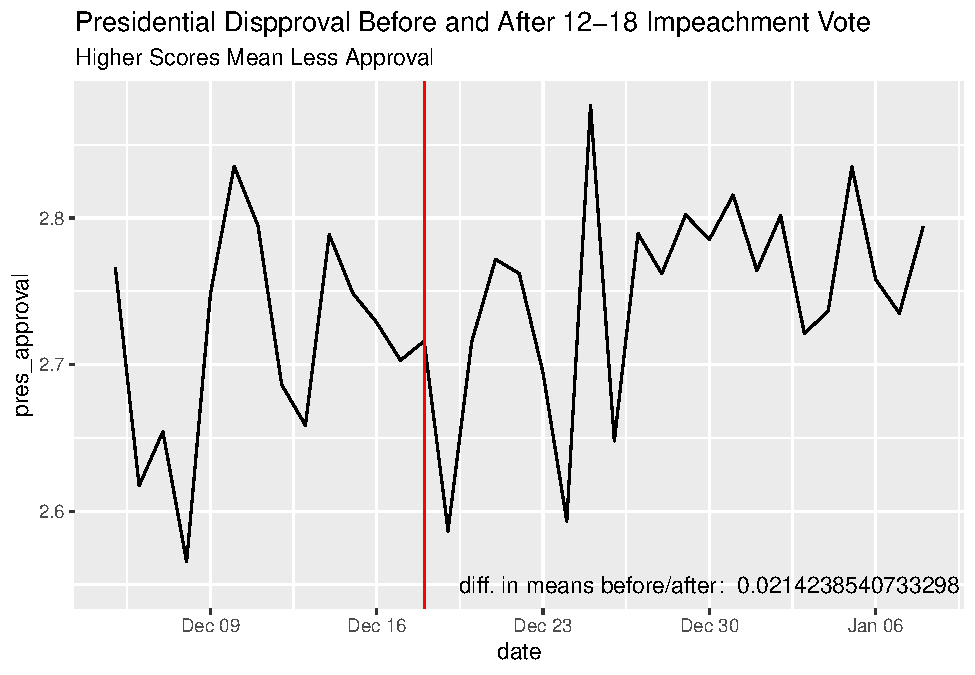
\includegraphics{data_assignment10_nov_11_2021_files/figure-latex/graphing-1.pdf}

\begin{Shaded}
\begin{Highlighting}[]
\NormalTok{consider_trump_graph}
\end{Highlighting}
\end{Shaded}

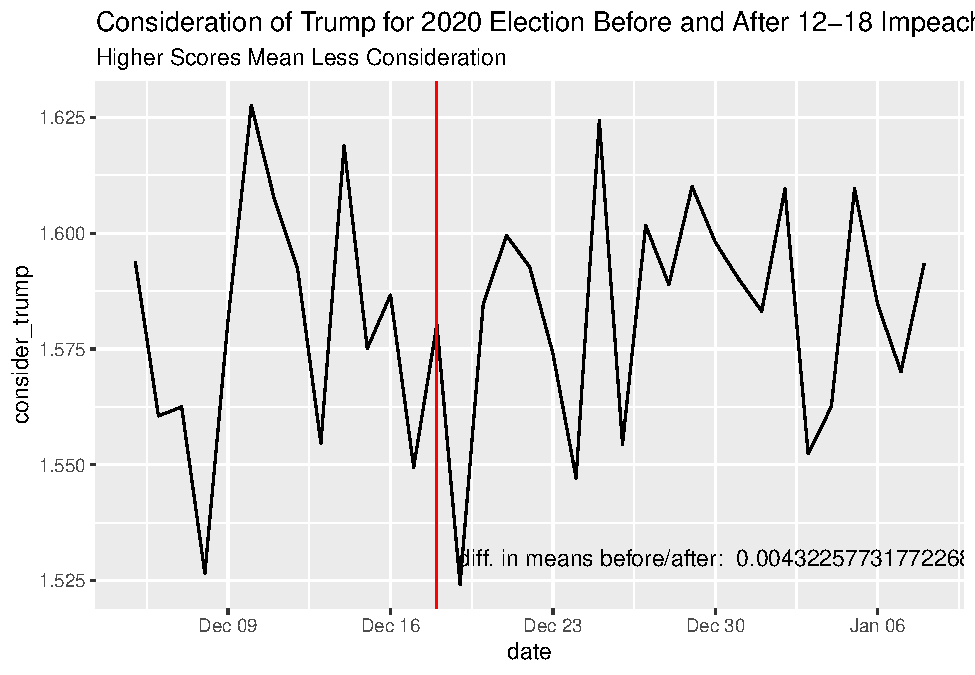
\includegraphics{data_assignment10_nov_11_2021_files/figure-latex/graphing-2.pdf}

\begin{Shaded}
\begin{Highlighting}[]
\NormalTok{pid7_legacy_graph}
\end{Highlighting}
\end{Shaded}

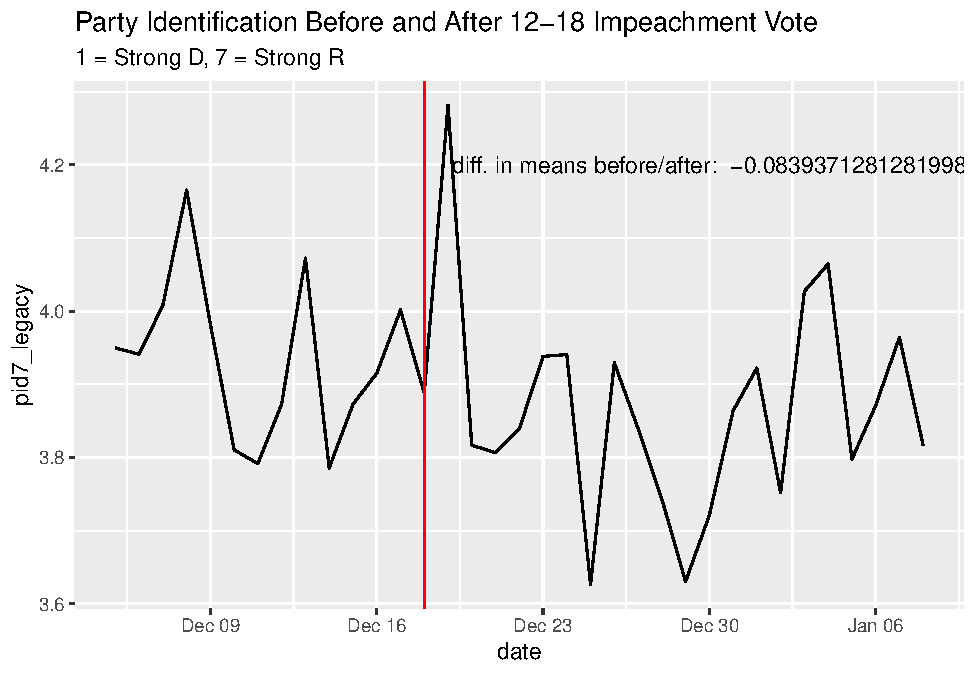
\includegraphics{data_assignment10_nov_11_2021_files/figure-latex/graphing-3.pdf}

\begin{Shaded}
\begin{Highlighting}[]
\NormalTok{ideo5_graph}
\end{Highlighting}
\end{Shaded}

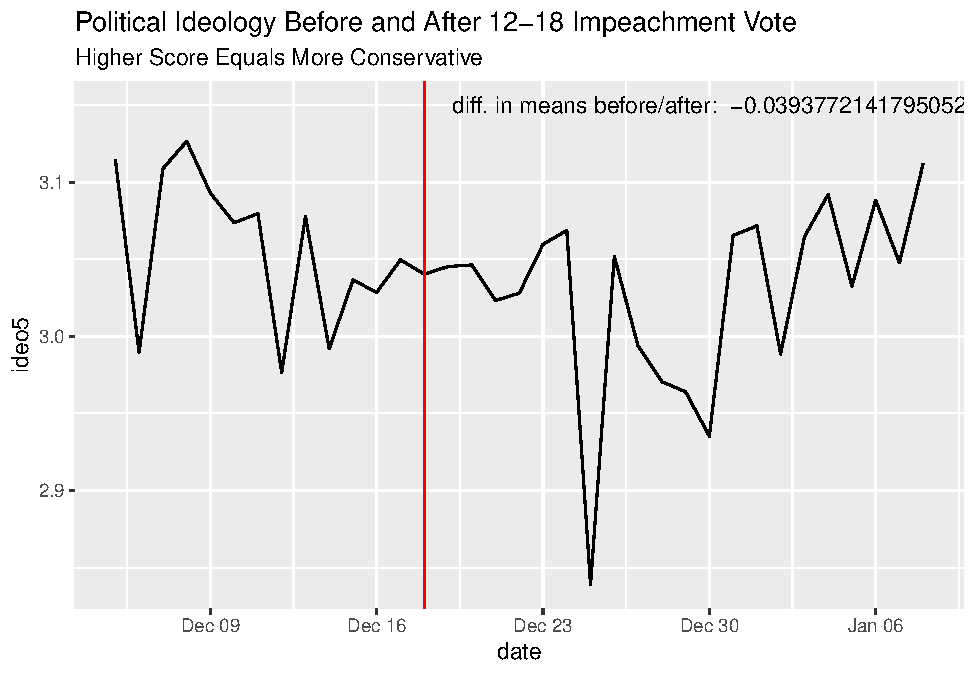
\includegraphics{data_assignment10_nov_11_2021_files/figure-latex/graphing-4.pdf}

\begin{Shaded}
\begin{Highlighting}[]
\NormalTok{muslimban_graph}
\end{Highlighting}
\end{Shaded}

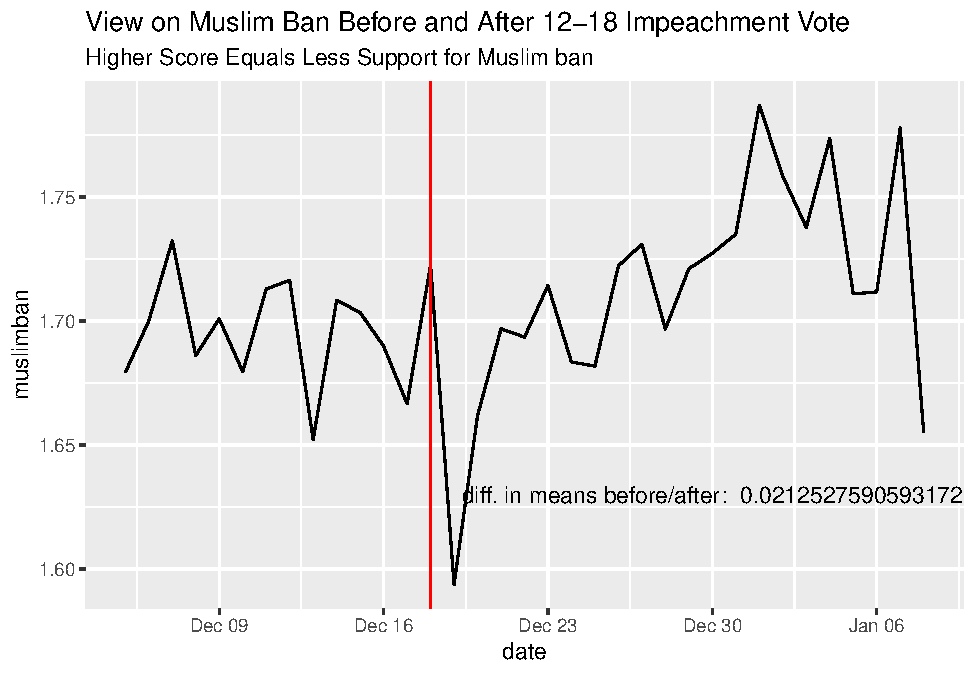
\includegraphics{data_assignment10_nov_11_2021_files/figure-latex/graphing-5.pdf}

\begin{Shaded}
\begin{Highlighting}[]
\KeywordTok{grid.arrange}\NormalTok{(pres_approval_graph, consider_trump_graph, pid7_legacy_graph, ideo5_graph, muslimban_graph)}
\end{Highlighting}
\end{Shaded}

\includegraphics{data_assignment10_nov_11_2021_files/figure-latex/graphing-6.pdf}

\hypertarget{question-7-data-science-question}{%
\subsection{Question 7: DATA SCIENCE
QUESTION}\label{question-7-data-science-question}}

\textbf{Extend your work from the previous question to consider other
factors, like the possibility of heterogenous treatment effects,
confounding variables, or use a more sophisticated approach to
statistical inference, like regression discontinuity in time.}

\begin{Shaded}
\begin{Highlighting}[]
\CommentTok{#running a standardized multiple regression}

\NormalTok{std_data <-}\StringTok{ }\NormalTok{full_data }\OperatorTok
\StringTok{  }\KeywordTok{mutate}\NormalTok{(}\DataTypeTok{standardized_pres_approval =} \KeywordTok{scale}\NormalTok{(pres_approval)) }\OperatorTok
\StringTok{  }\KeywordTok{mutate}\NormalTok{(}\DataTypeTok{standardized_consider_trump =} \KeywordTok{scale}\NormalTok{(consider_trump)) }\OperatorTok
\StringTok{  }\KeywordTok{mutate}\NormalTok{(}\DataTypeTok{standardized_pid7_legacy =} \KeywordTok{scale}\NormalTok{(pid7_legacy)) }\OperatorTok
\StringTok{  }\KeywordTok{mutate}\NormalTok{(}\DataTypeTok{standardized_ideo5 =} \KeywordTok{scale}\NormalTok{(ideo5)) }\OperatorTok
\StringTok{  }\KeywordTok{mutate}\NormalTok{(}\DataTypeTok{standardized_muslimban =} \KeywordTok{scale}\NormalTok{(muslimban)) }\OperatorTok
\StringTok{  }\KeywordTok{mutate}\NormalTok{(}\DataTypeTok{standardized_age =} \KeywordTok{scale}\NormalTok{(age)) }\OperatorTok
\StringTok{  }\KeywordTok{mutate}\NormalTok{(}\DataTypeTok{standardized_witnessed_bc_imp =} \KeywordTok{scale}\NormalTok{(witnessed_bc_imp)) }\OperatorTok
\StringTok{  }\KeywordTok{mutate}\NormalTok{(}\DataTypeTok{standardized_treated =} \KeywordTok{scale}\NormalTok{(treated)) }\OperatorTok
\StringTok{  }\KeywordTok{select}\NormalTok{(standardized_pres_approval, standardized_consider_trump, standardized_pid7_legacy, standardized_ideo5, standardized_muslimban, standardized_age, standardized_witnessed_bc_imp, standardized_treated)}


\NormalTok{mr_model <-}\StringTok{ }\KeywordTok{lm}\NormalTok{(standardized_pid7_legacy }\OperatorTok{~}\StringTok{ }\NormalTok{standardized_treated }\OperatorTok{+}\StringTok{ }\NormalTok{standardized_pres_approval }\OperatorTok{+}\StringTok{ }\NormalTok{standardized_consider_trump }\OperatorTok{+}\StringTok{ }\NormalTok{standardized_ideo5 }\OperatorTok{+}\StringTok{ }\NormalTok{standardized_muslimban }\OperatorTok{+}\StringTok{ }\NormalTok{standardized_age }\OperatorTok{+}\StringTok{ }\NormalTok{standardized_witnessed_bc_imp, }\DataTypeTok{data =}\NormalTok{ std_data)}

\KeywordTok{plot_summs}\NormalTok{(mr_model, }\DataTypeTok{scale =} \OtherTok{TRUE}\NormalTok{, }\DataTypeTok{inner_ci_level =} \FloatTok{.9}\NormalTok{) }\OperatorTok{+}
\StringTok{  }\KeywordTok{labs}\NormalTok{(}\DataTypeTok{title =} \StringTok{"Multiple Regression Estimates of Effect on PID7"}\NormalTok{)}
\end{Highlighting}
\end{Shaded}

\begin{verbatim}
## Loading required namespace: broom.mixed
## Loading required namespace: broom.mixed
\end{verbatim}

\includegraphics{data_assignment10_nov_11_2021_files/figure-latex/multiple_regression-1.pdf}

\end{document}
